%------------------------------------------------------------------------------
\chapter{Thin Sensors}
\label{sec:appendix_ThinSensors}
%------------------------------------------------------------------------------

%% --------------------------------------------- %%
\section{Depletion voltage}

\begin{figure}[htbp] \centering
  \begin{subfigure}[b]{0.33\textwidth}
    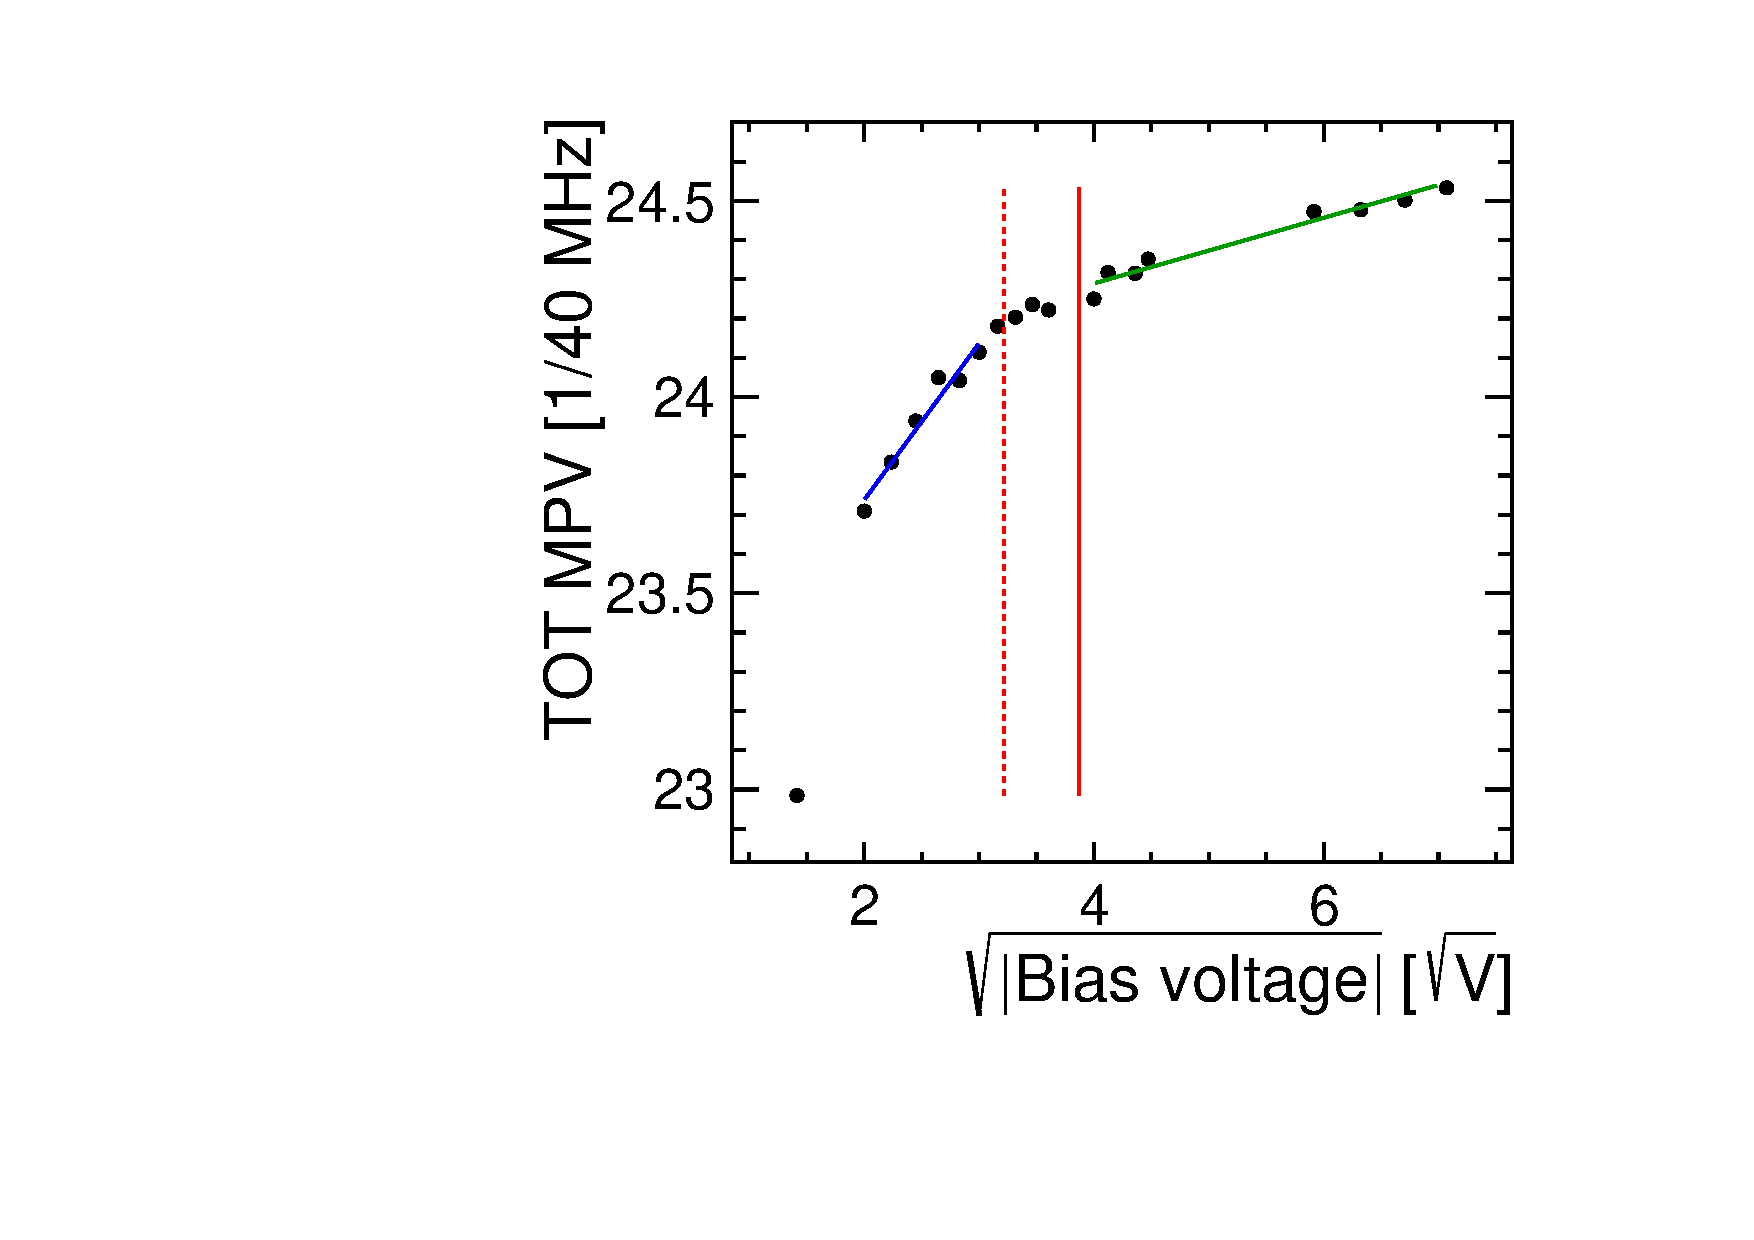
\includegraphics[width=\textwidth]{./figures/TestBeam/depletionVoltage_W0019_G07.pdf}
    \caption{20-NGR}
  \end{subfigure} \hfill
  \begin{subfigure}[b]{0.33\textwidth}
    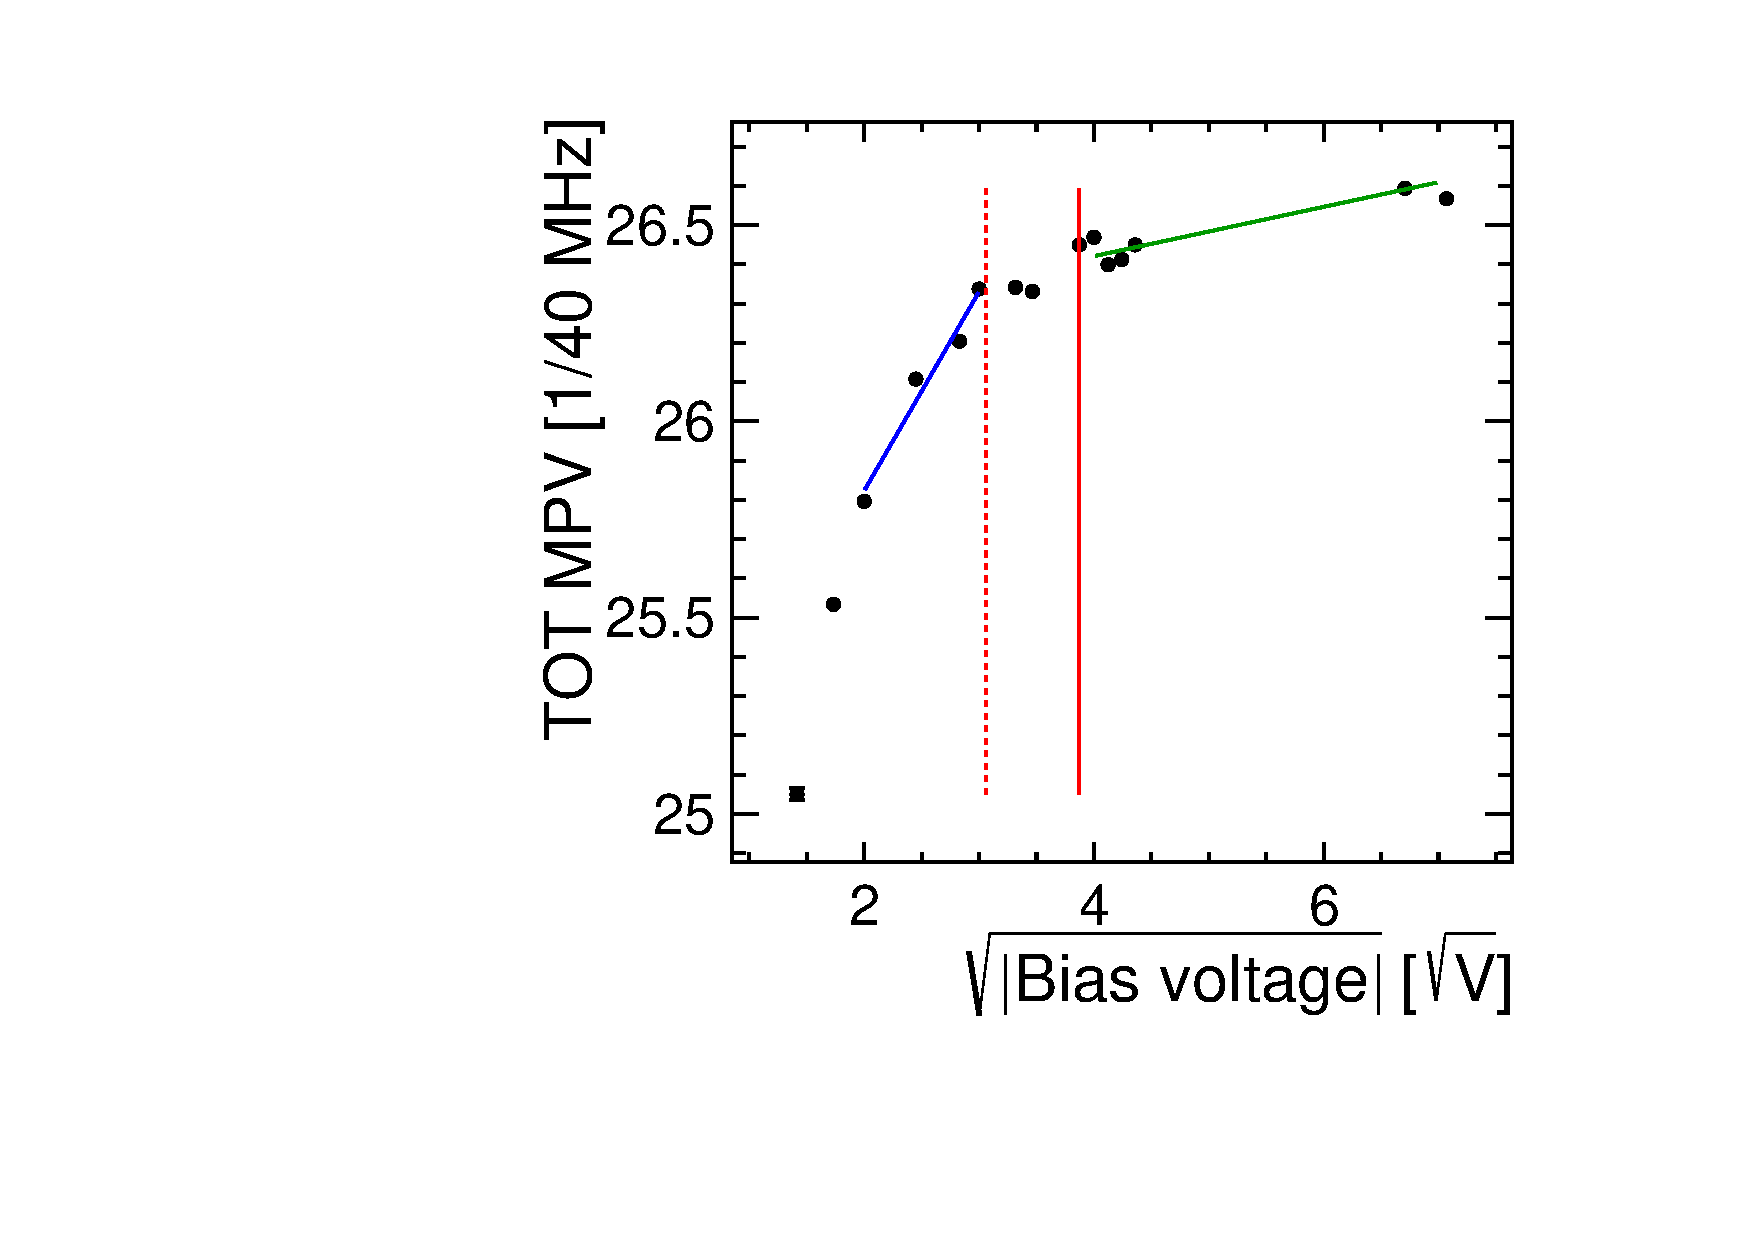
\includegraphics[width=\textwidth]{./figures/TestBeam/depletionVoltage_W0019_F07.pdf}
    \caption{23-FGR}
  \end{subfigure}\hfill
  \begin{subfigure}[b]{0.33\textwidth}
    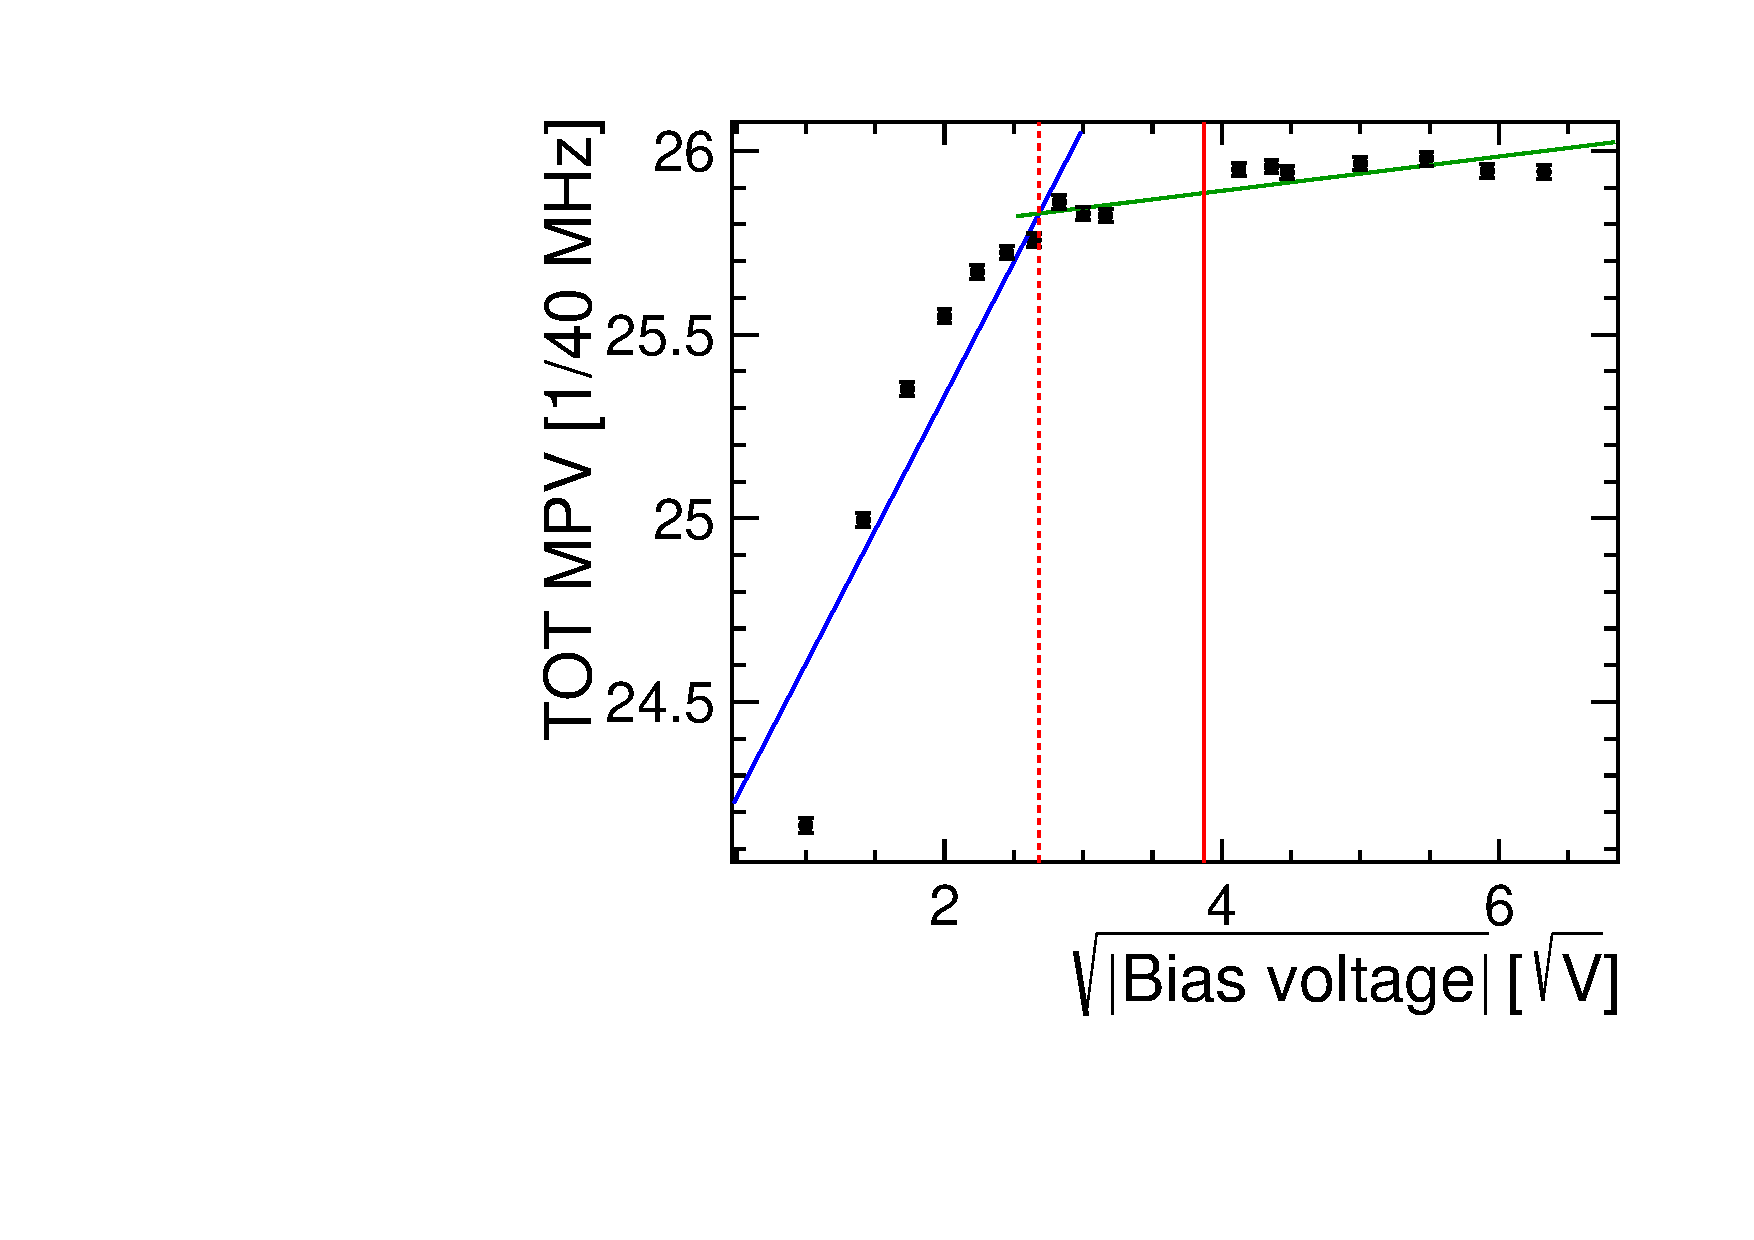
\includegraphics[width=\textwidth]{./figures/TestBeam/depletionVoltage_W0019_L08.pdf}
    \caption{28-GNDGR}
  \end{subfigure} \\

  \begin{subfigure}[b]{0.33\textwidth}
    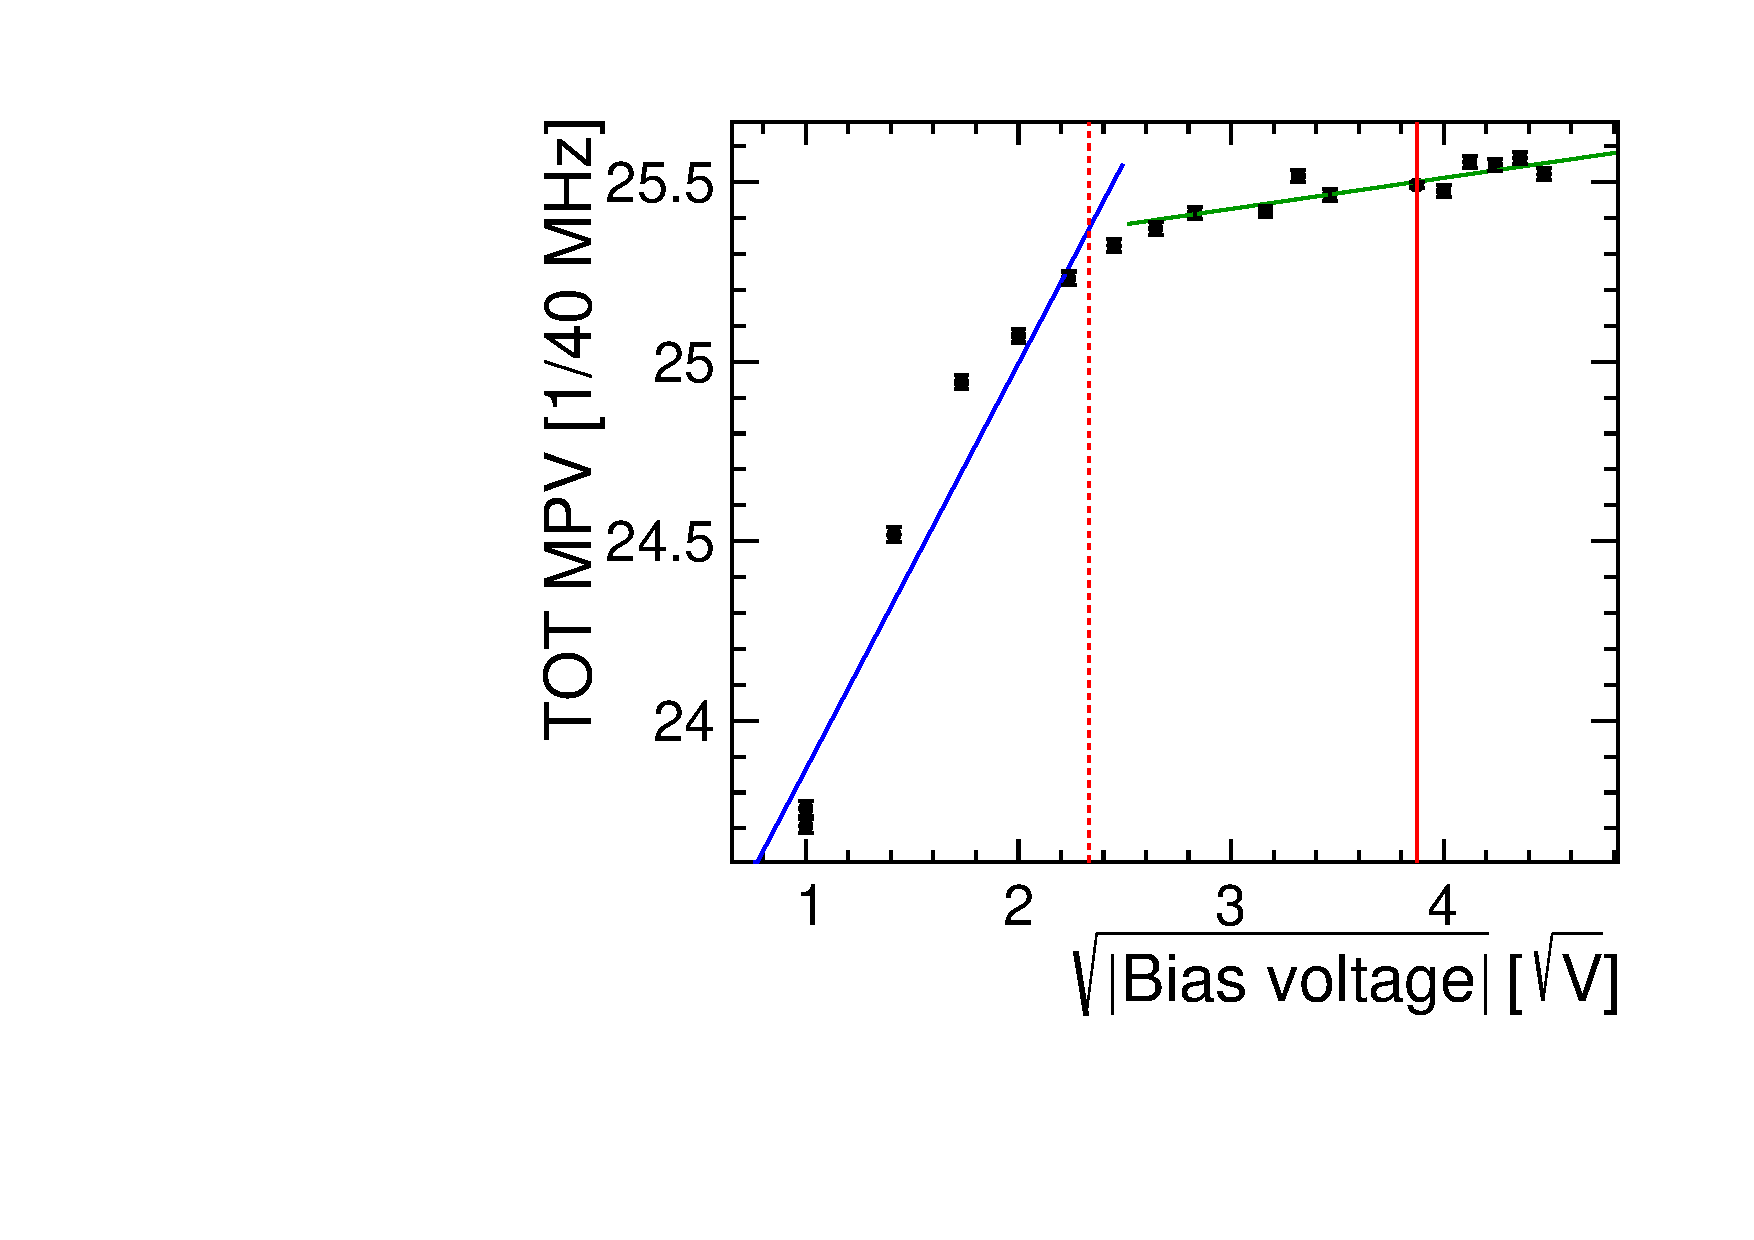
\includegraphics[width=\textwidth]{./figures/TestBeam/depletionVoltage_W0019_C07.pdf}
    \caption{55-GNDGR}
  \end{subfigure} \hfill
  \begin{subfigure}[b]{0.33\textwidth}
    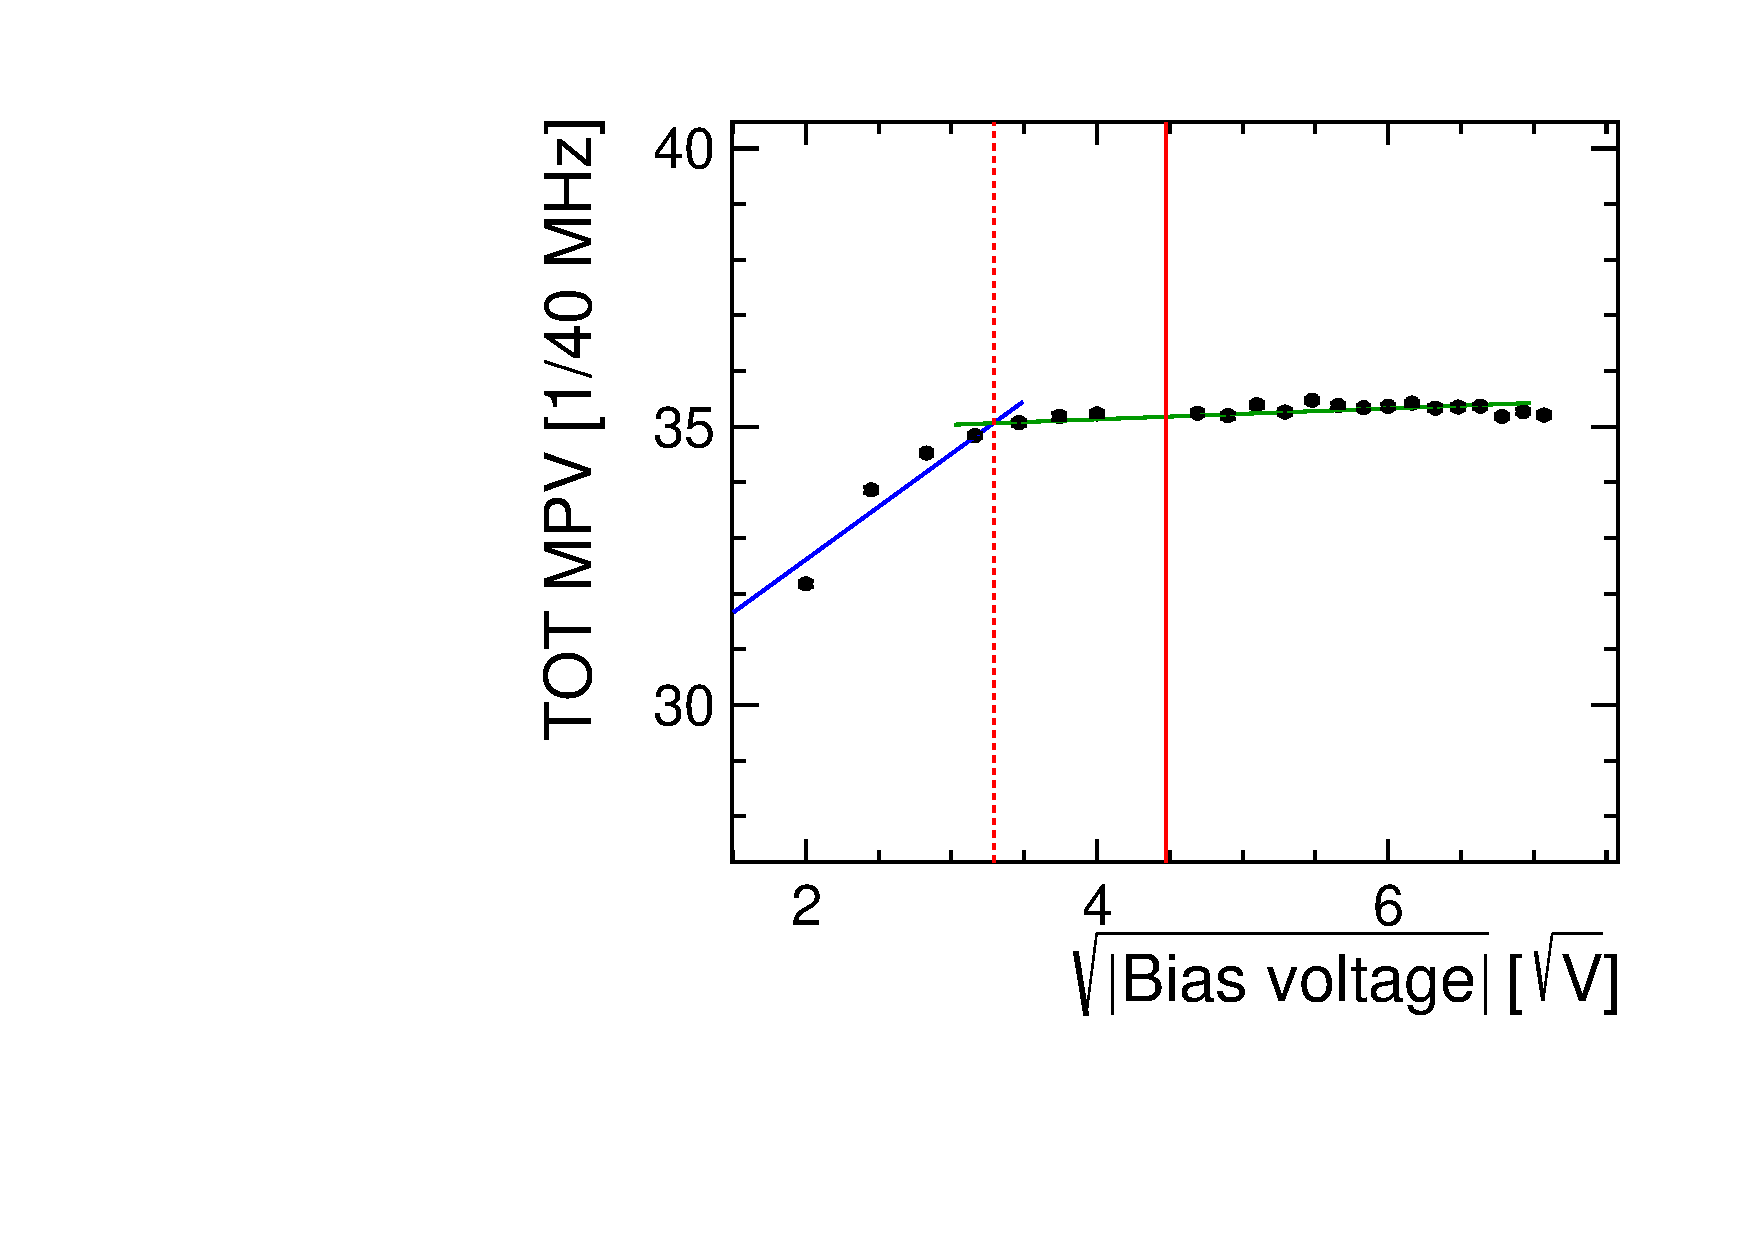
\includegraphics[width=\textwidth]{./figures/TestBeam/depletionVoltage_W0005_E02.pdf}
    \caption{55-GND-GR-100}
  \end{subfigure}\hfill
  \begin{subfigure}[b]{0.33\textwidth}
    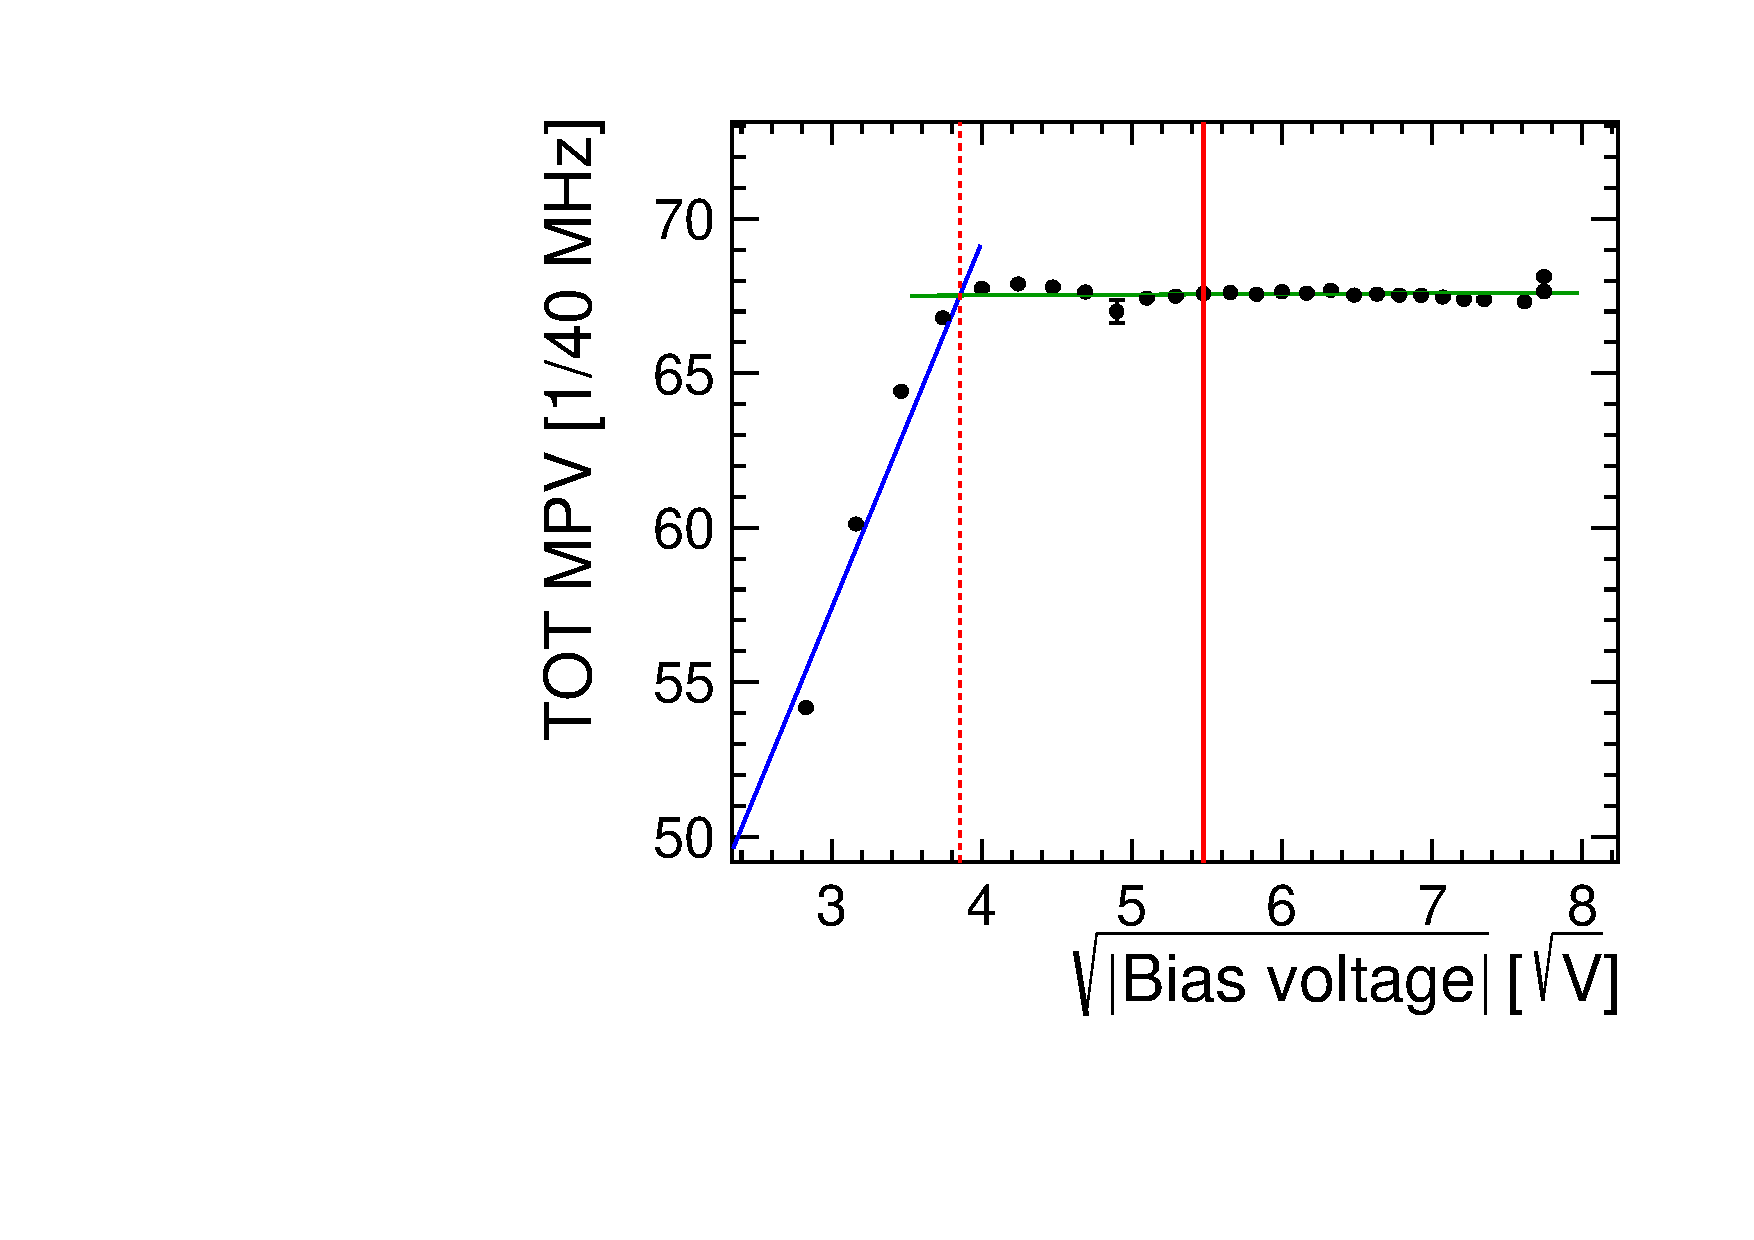
\includegraphics[width=\textwidth]{./figures/TestBeam/depletionVoltage_W0005_F01.pdf}
    \caption{55-GND-GR-150}
  \end{subfigure}\\
  \begin{subfigure}[b]{0.33\textwidth}
    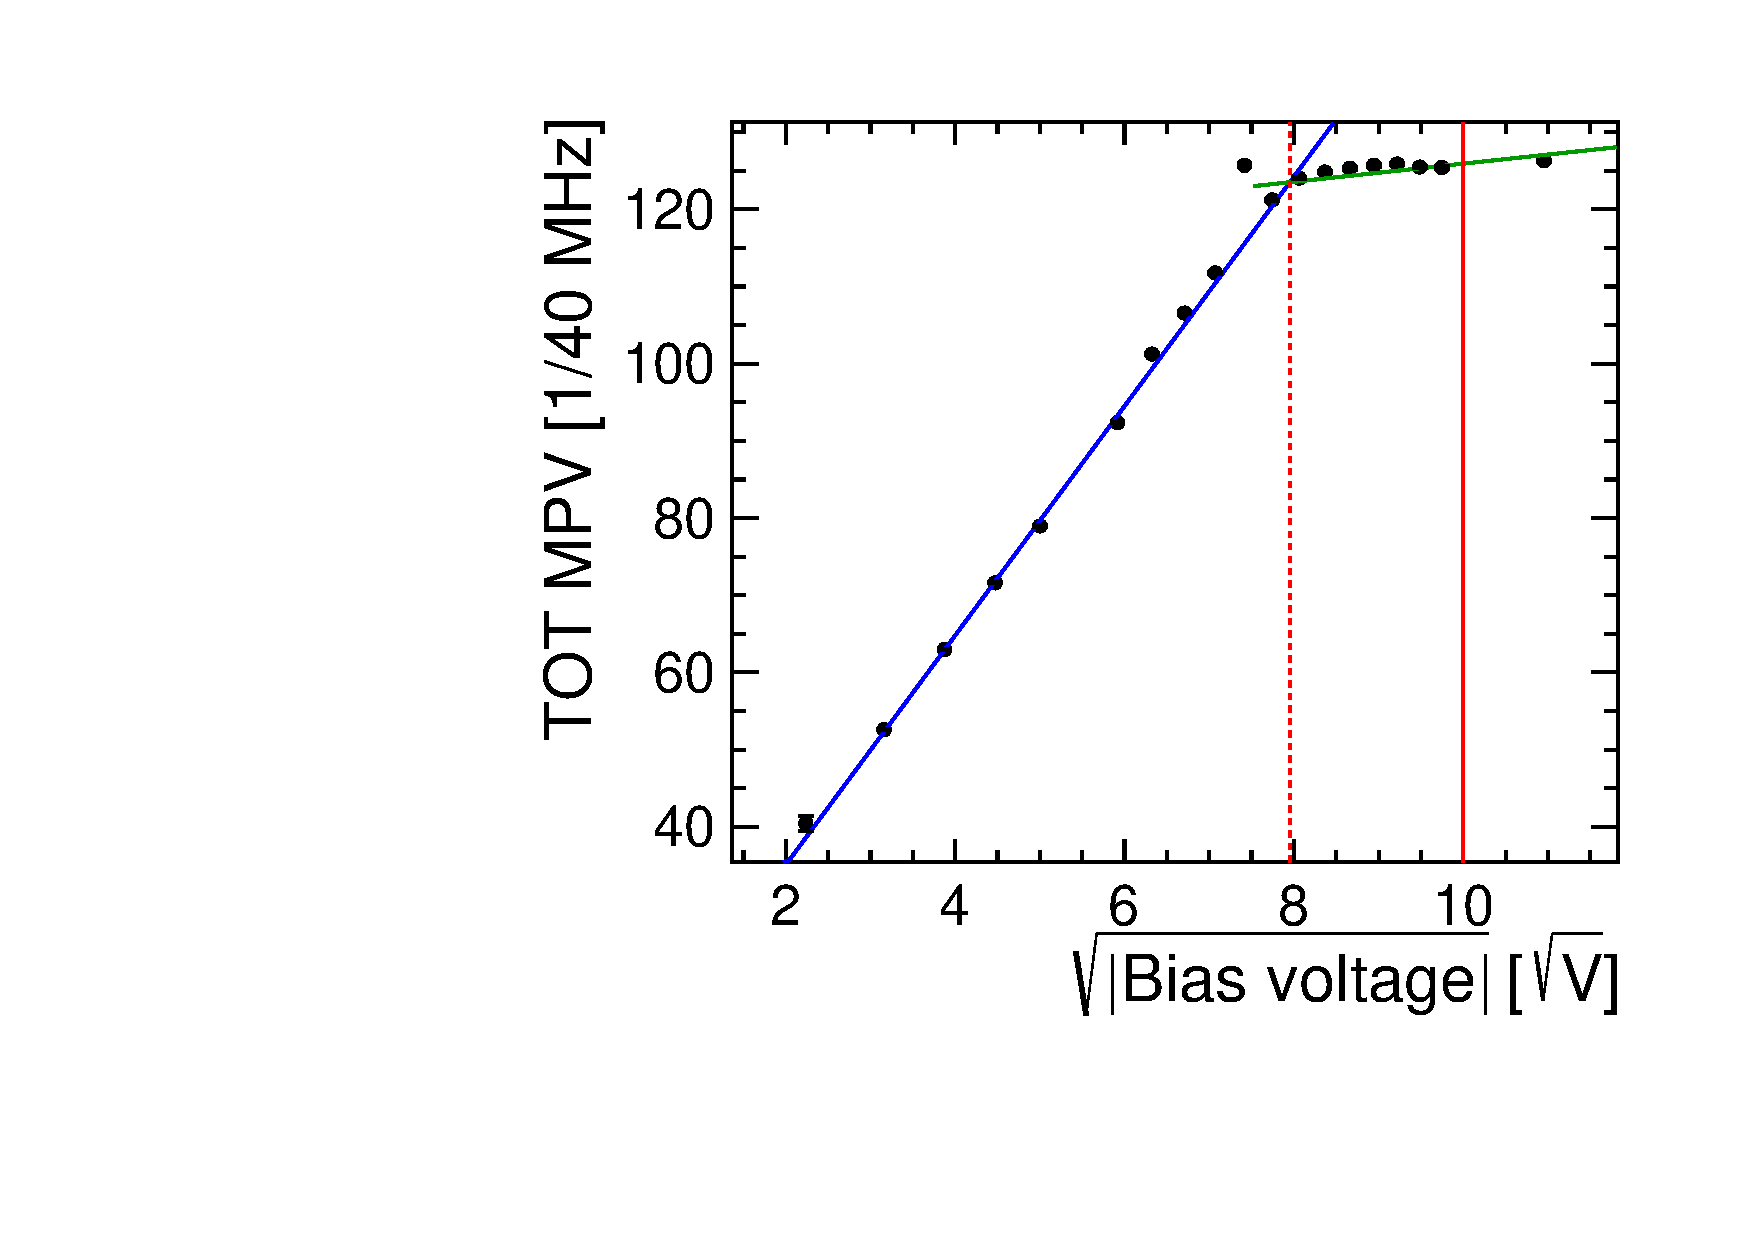
\includegraphics[width=\textwidth]{./figures/TestBeam/depletionVoltage_W0002_J05.pdf}
    \caption{W2\_J5}
  \end{subfigure}
  \caption{The depletion voltage is shown in dashed line and the nominal operating voltage is shown in continuous line.}
  \label{fig:depletionVoltage}
\end{figure}

\newpage
%% --------------------------------------------- %%
\section{Cluster size distribution}
\subsection{Cluster size vs. bias voltage}
\begin{figure}[htbp] \centering
  \begin{subfigure}[b]{0.33\textwidth}
    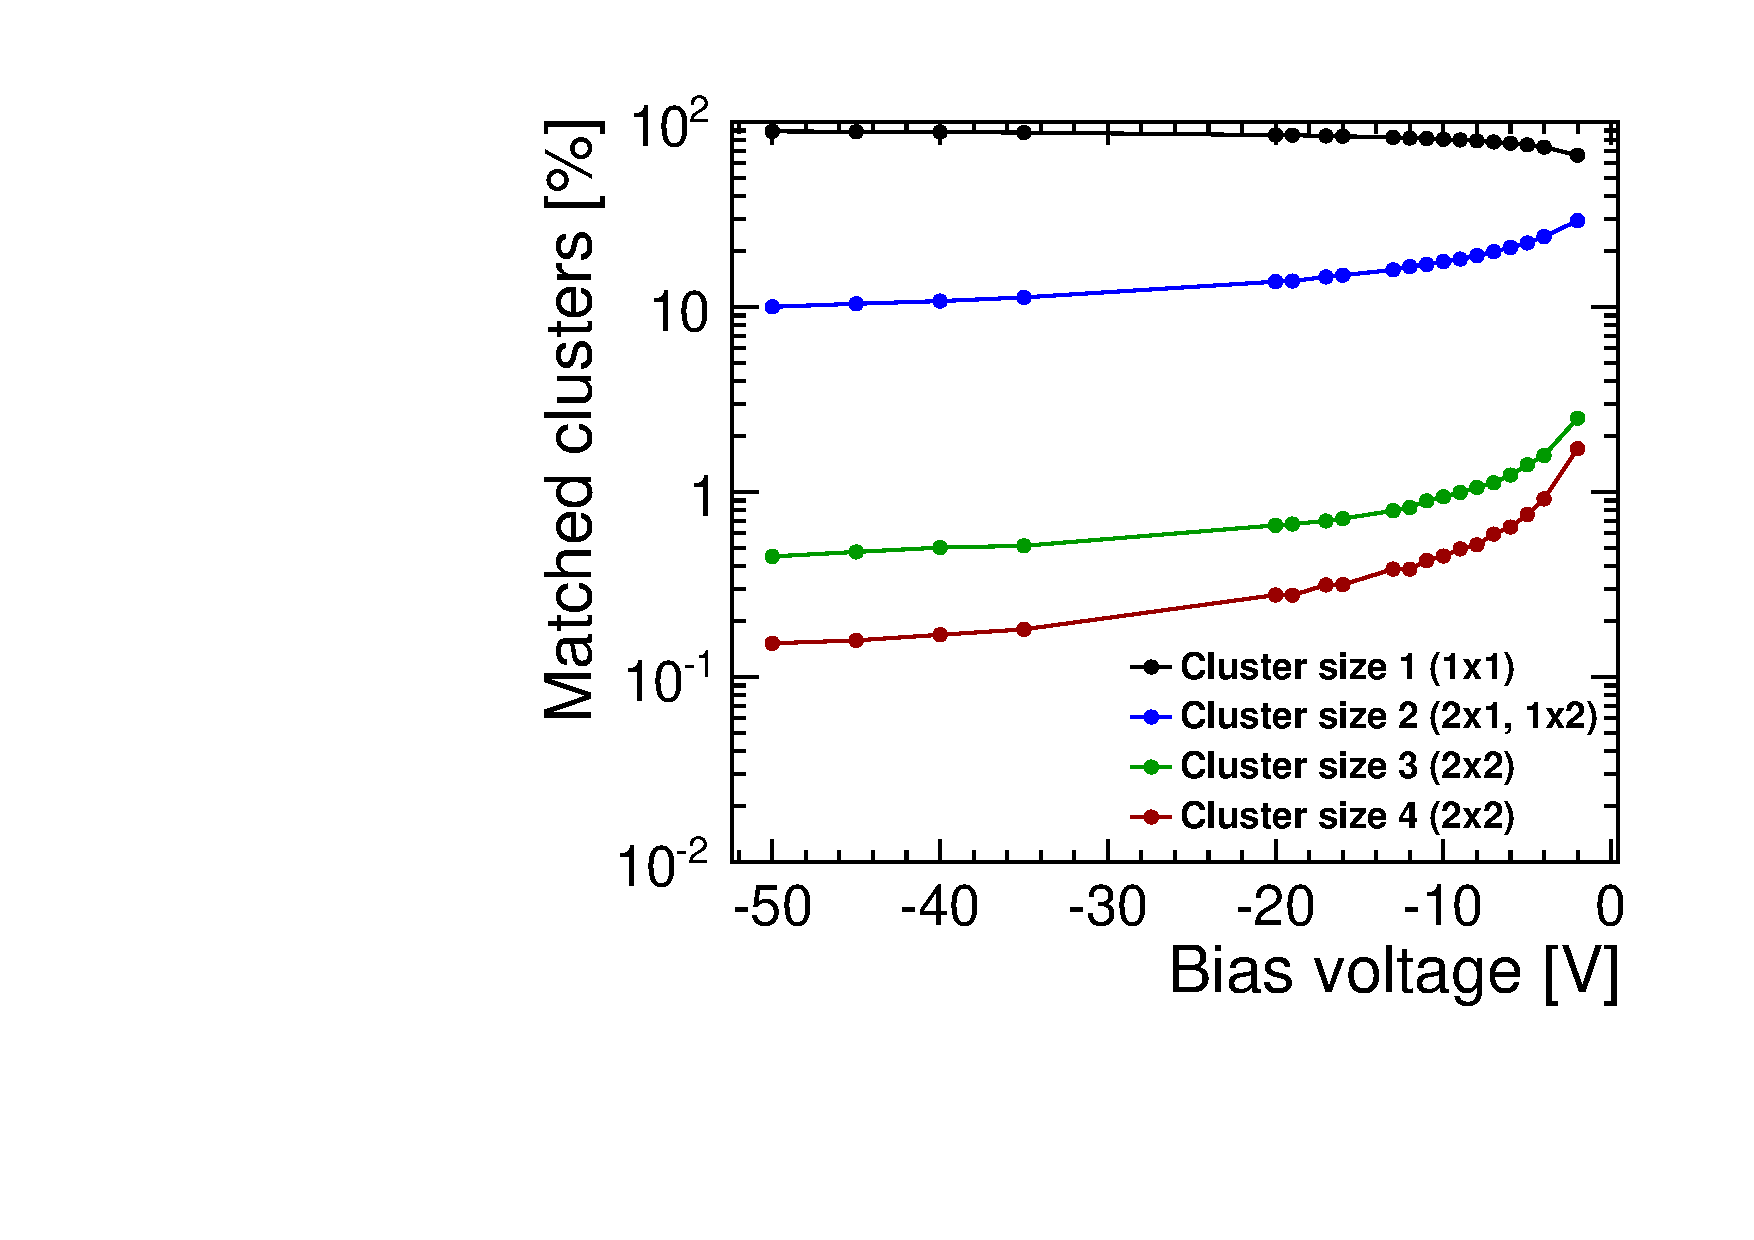
\includegraphics[width=\textwidth]{./figures/TestBeam/cluSize_biasScan_W0019_G07.pdf}
    \caption{20-NGR}
  \end{subfigure} \hfill
  \begin{subfigure}[b]{0.33\textwidth}
    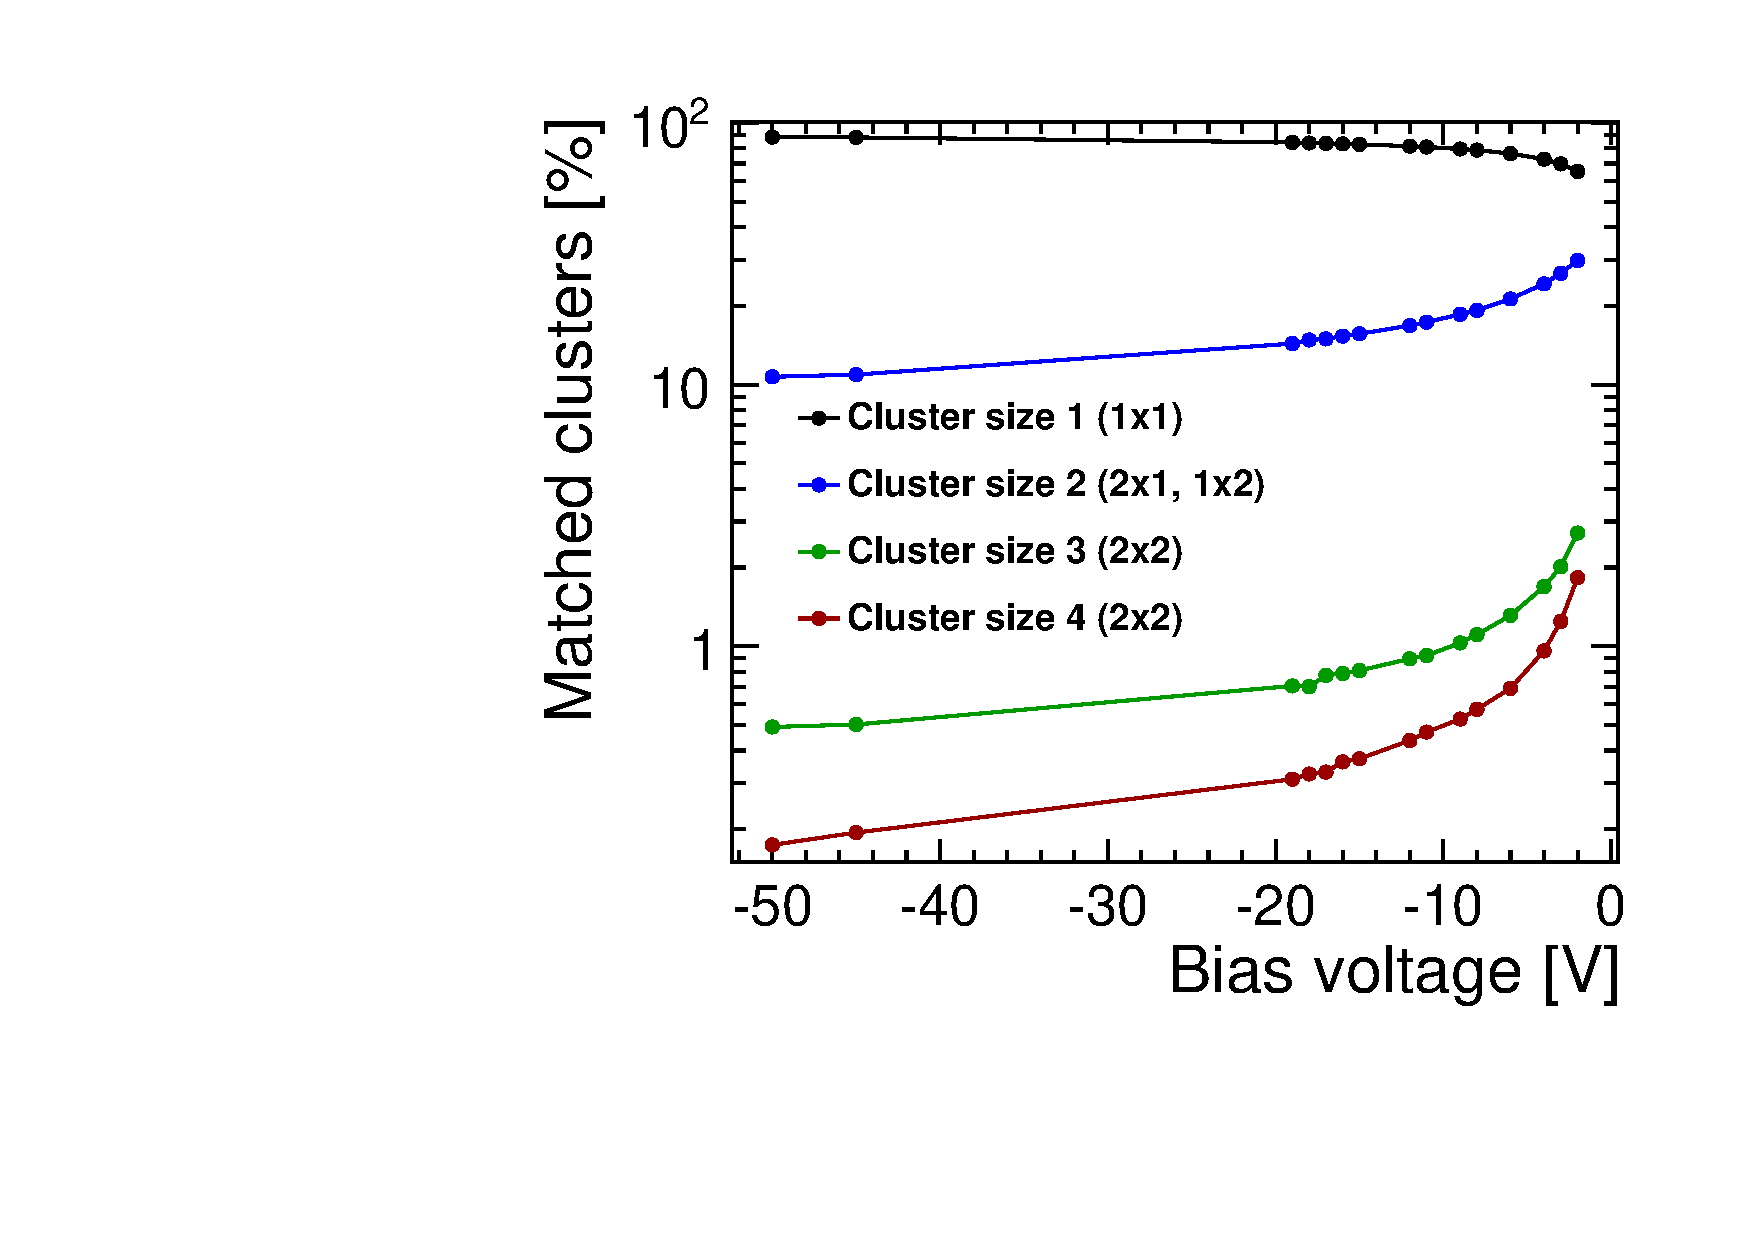
\includegraphics[width=\textwidth]{./figures/TestBeam/cluSize_biasScan_W0019_F07.pdf}
    \caption{23-FGR}
  \end{subfigure}\hfill
  \begin{subfigure}[b]{0.33\textwidth}
    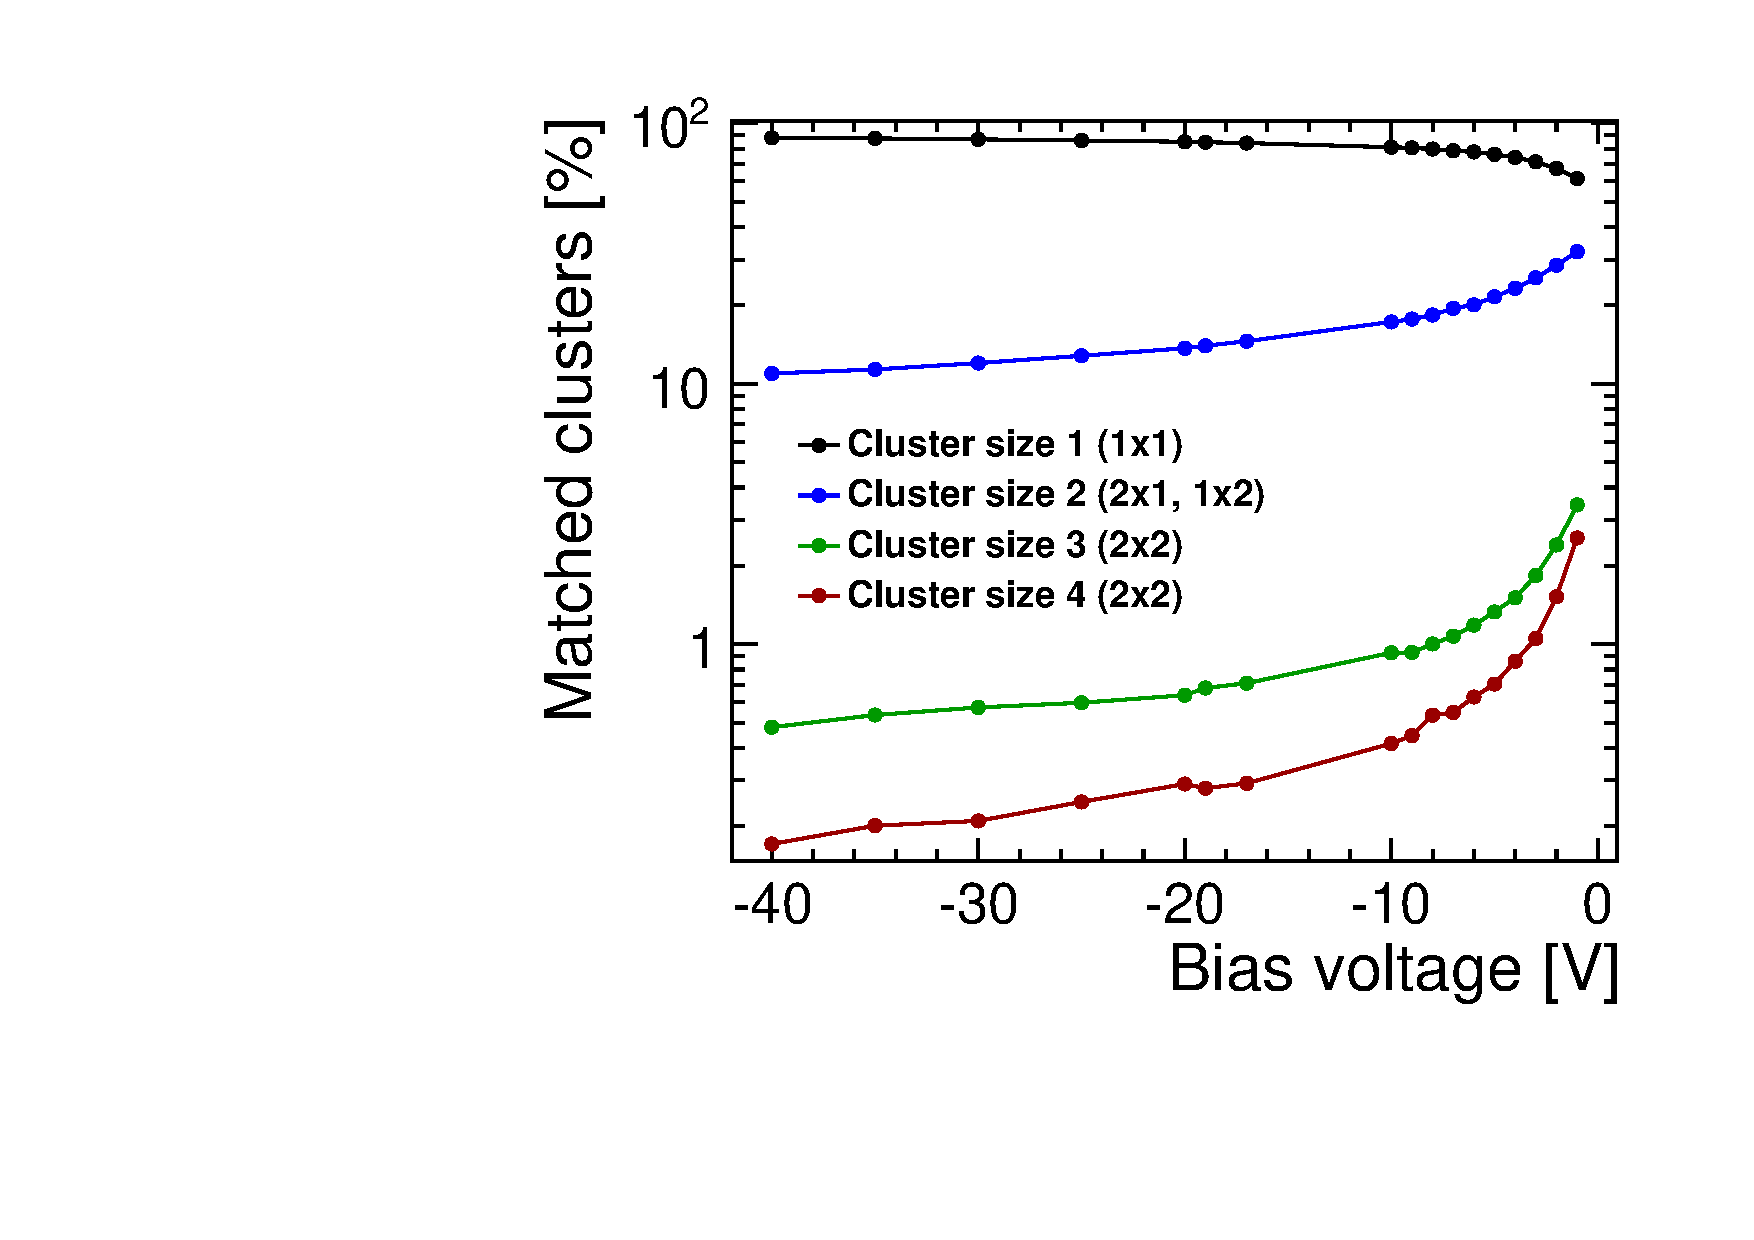
\includegraphics[width=\textwidth]{./figures/TestBeam/cluSize_biasScan_W0019_L08.pdf}
    \caption{28-GNDGR}
  \end{subfigure} \\

  \begin{subfigure}[b]{0.33\textwidth}
    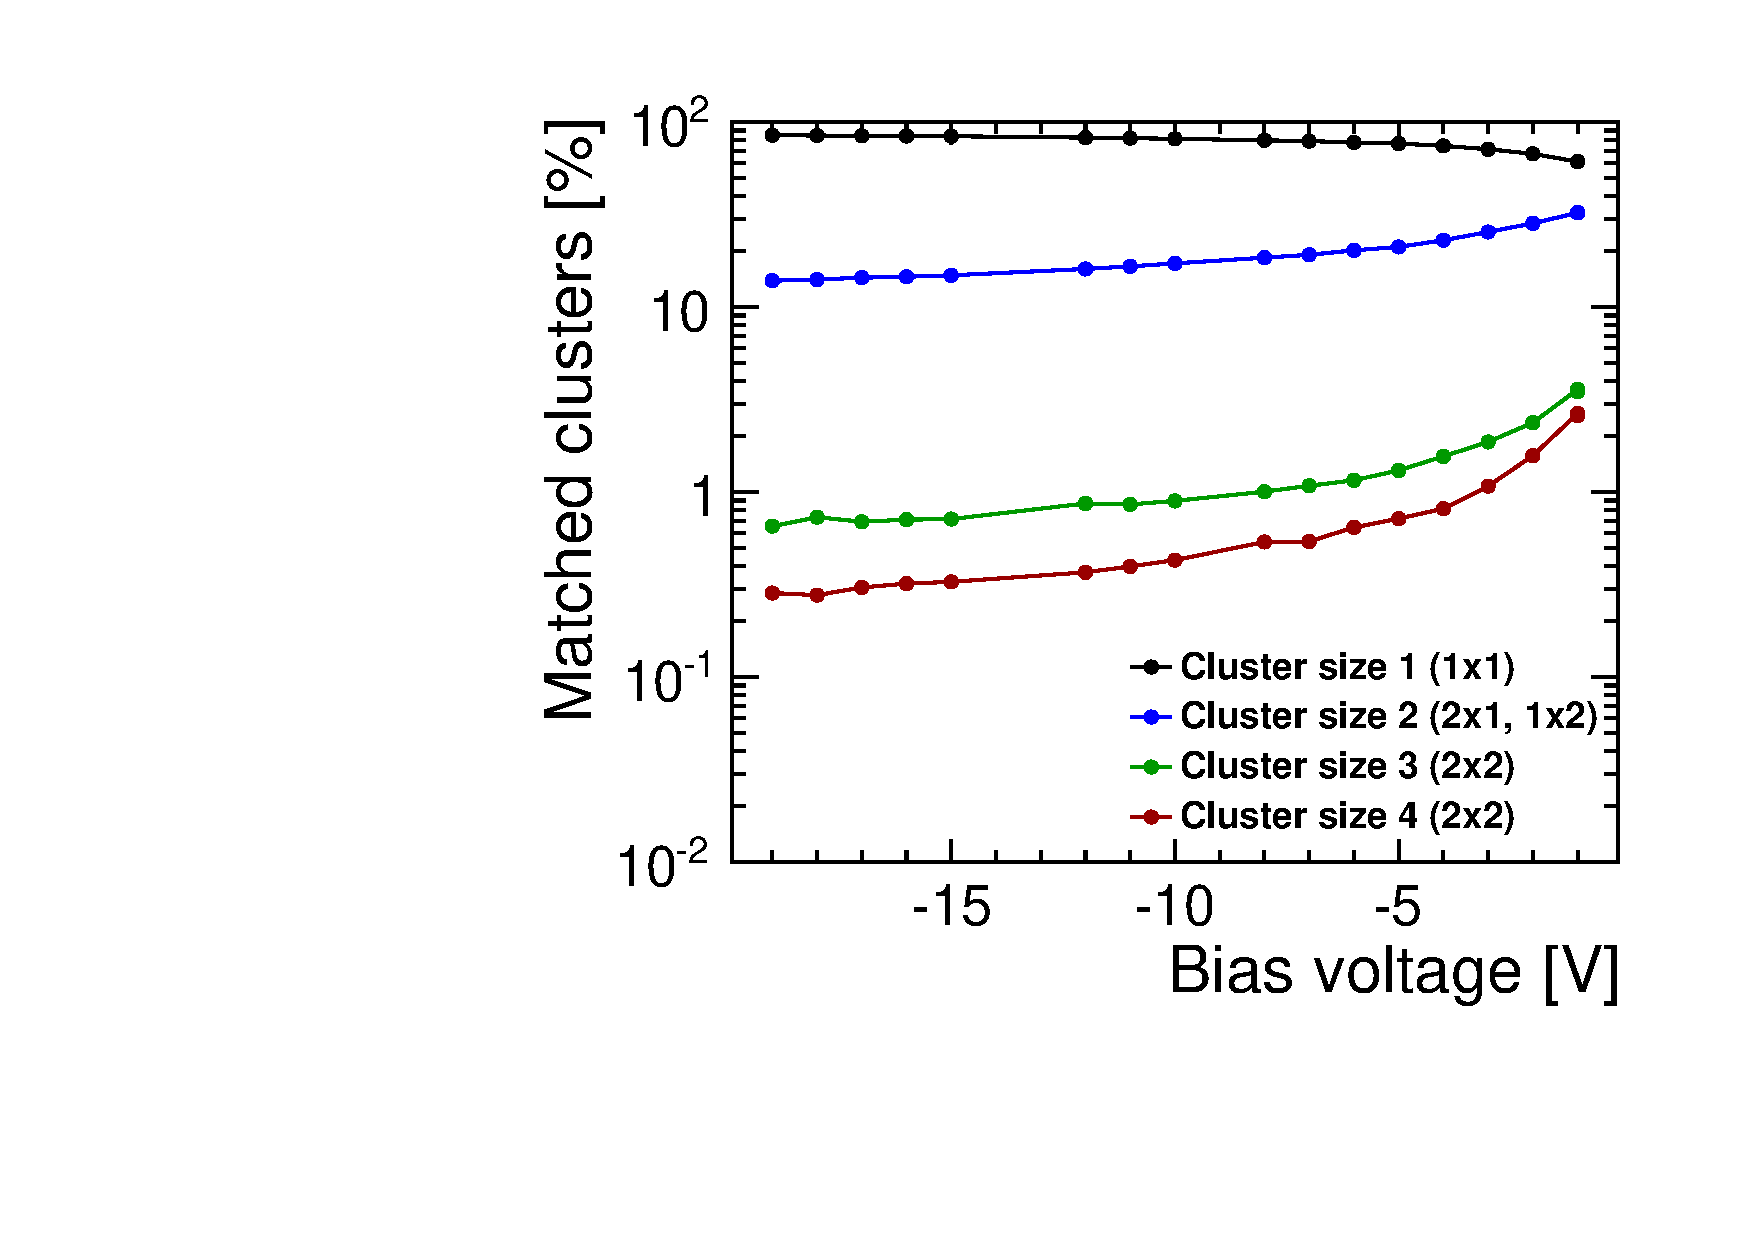
\includegraphics[width=\textwidth]{./figures/TestBeam/cluSize_biasScan_W0019_C07.pdf}
    \caption{55-GNDGR}
  \end{subfigure} \hfill
  \begin{subfigure}[b]{0.33\textwidth}
    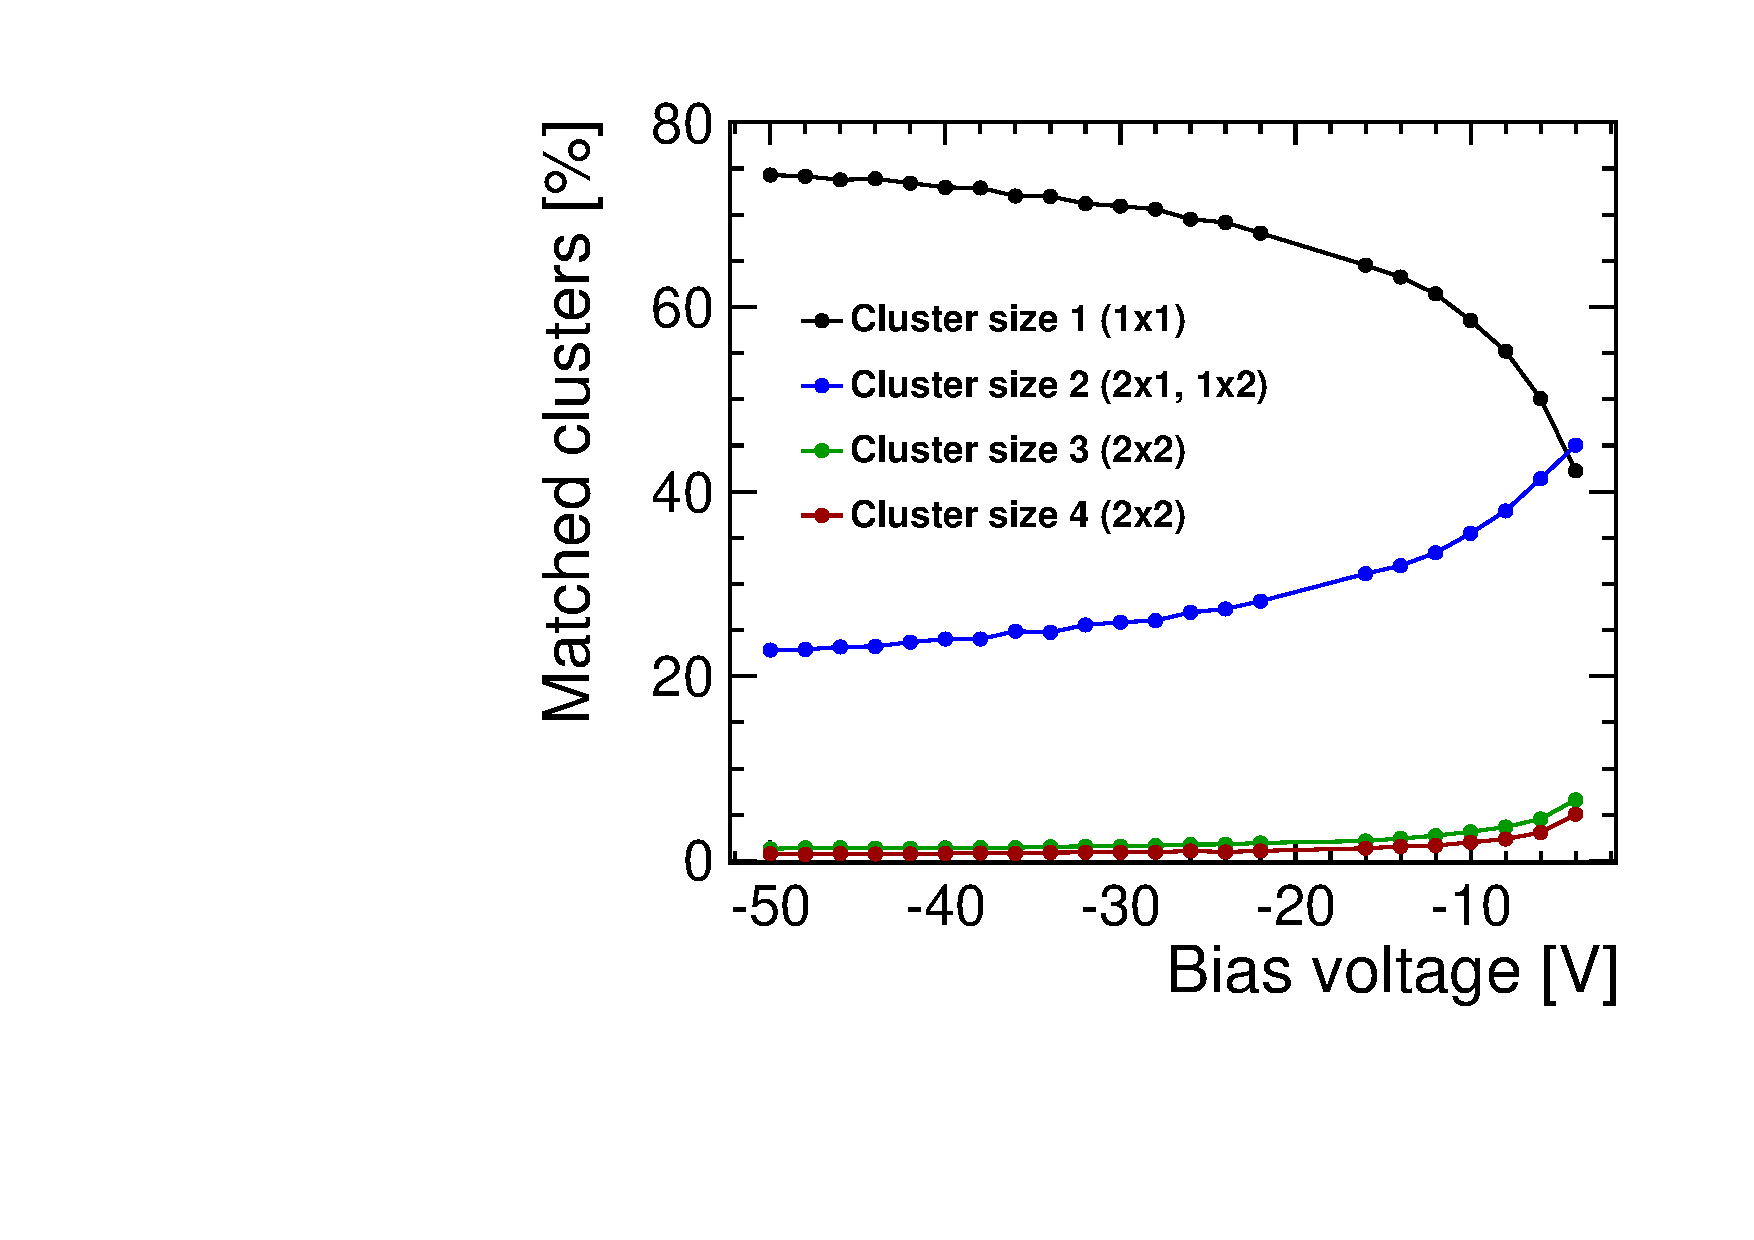
\includegraphics[width=\textwidth]{./figures/TestBeam/cluSize_biasScan_W0005_E02.pdf}
    \caption{55-GND-GR-100}
  \end{subfigure}\hfill
  \begin{subfigure}[b]{0.33\textwidth}
    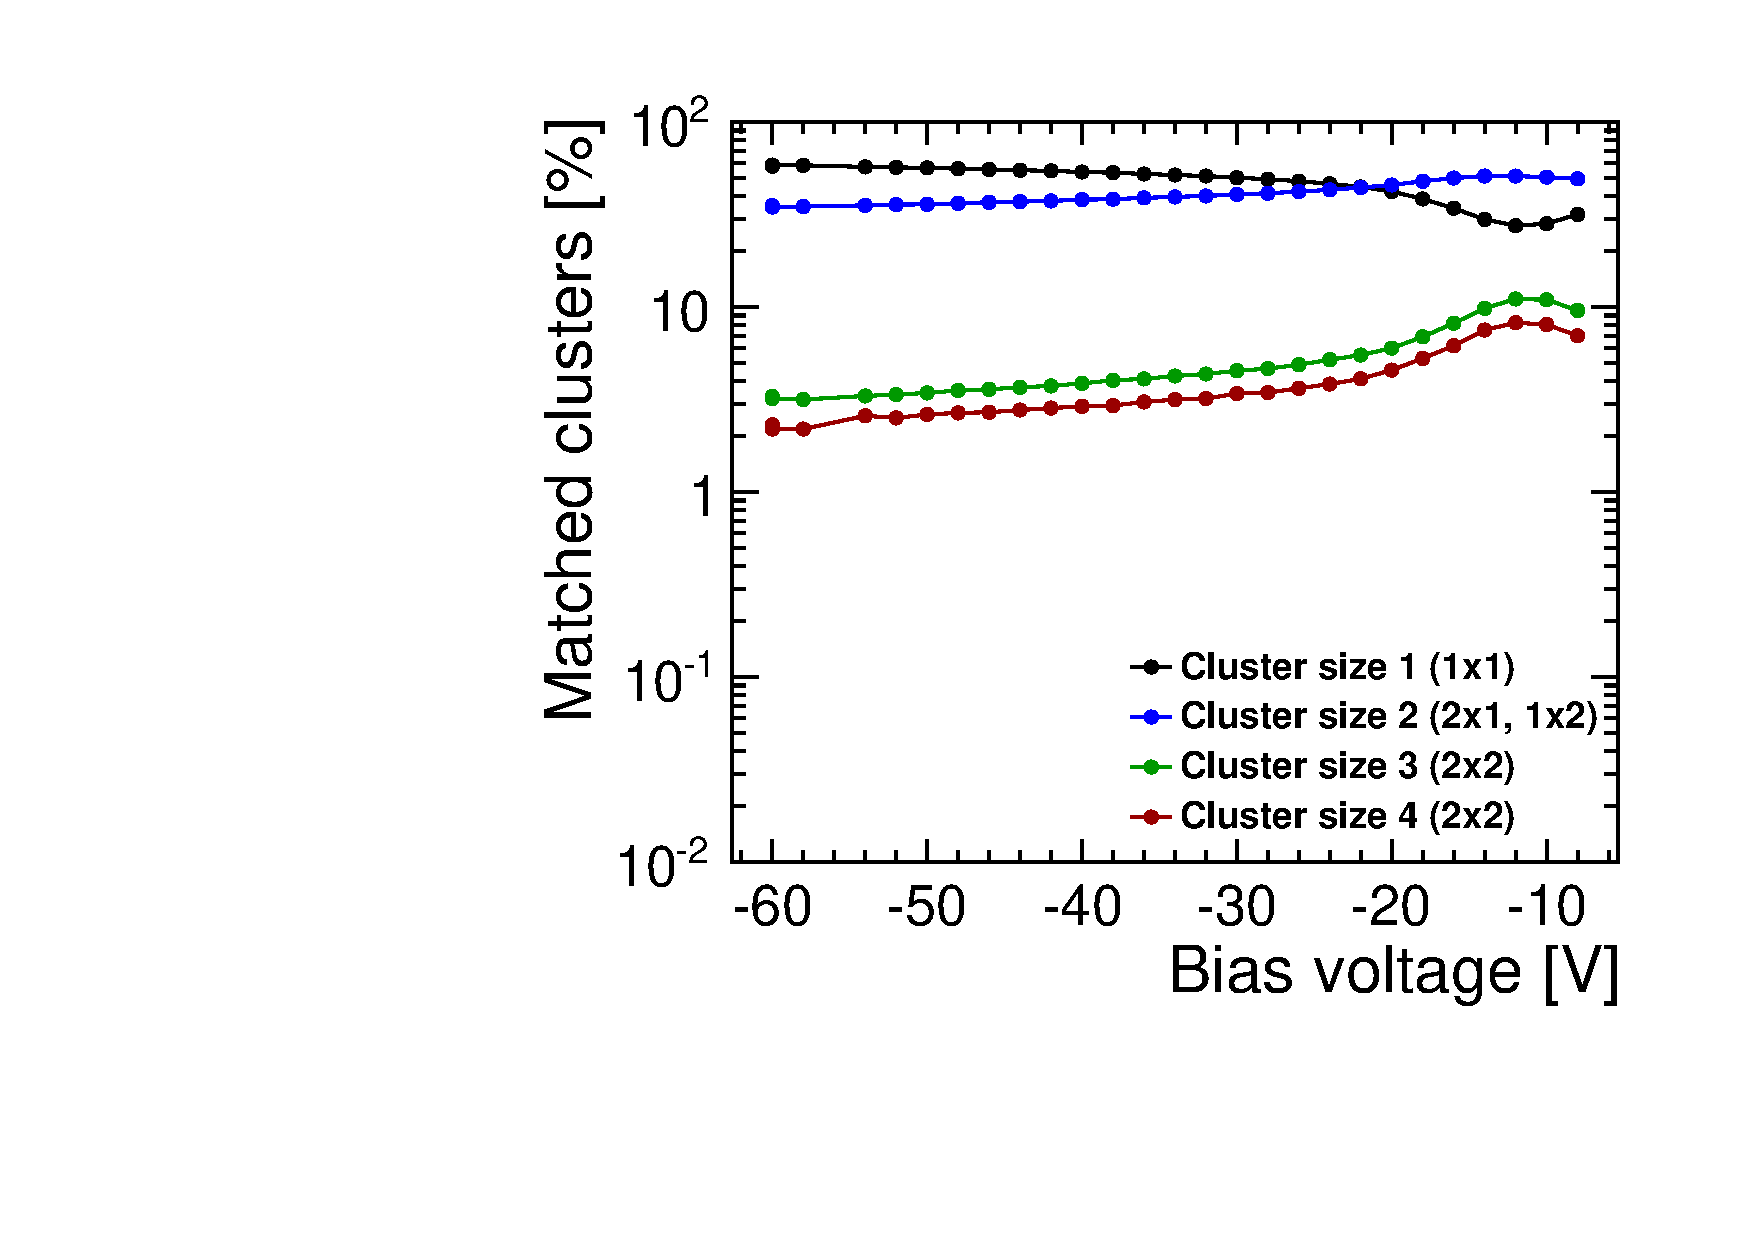
\includegraphics[width=\textwidth]{./figures/TestBeam/cluSize_biasScan_W0005_F01.pdf}
    \caption{55-GND-GR-150}
  \end{subfigure}\\
  \begin{subfigure}[b]{0.33\textwidth}
    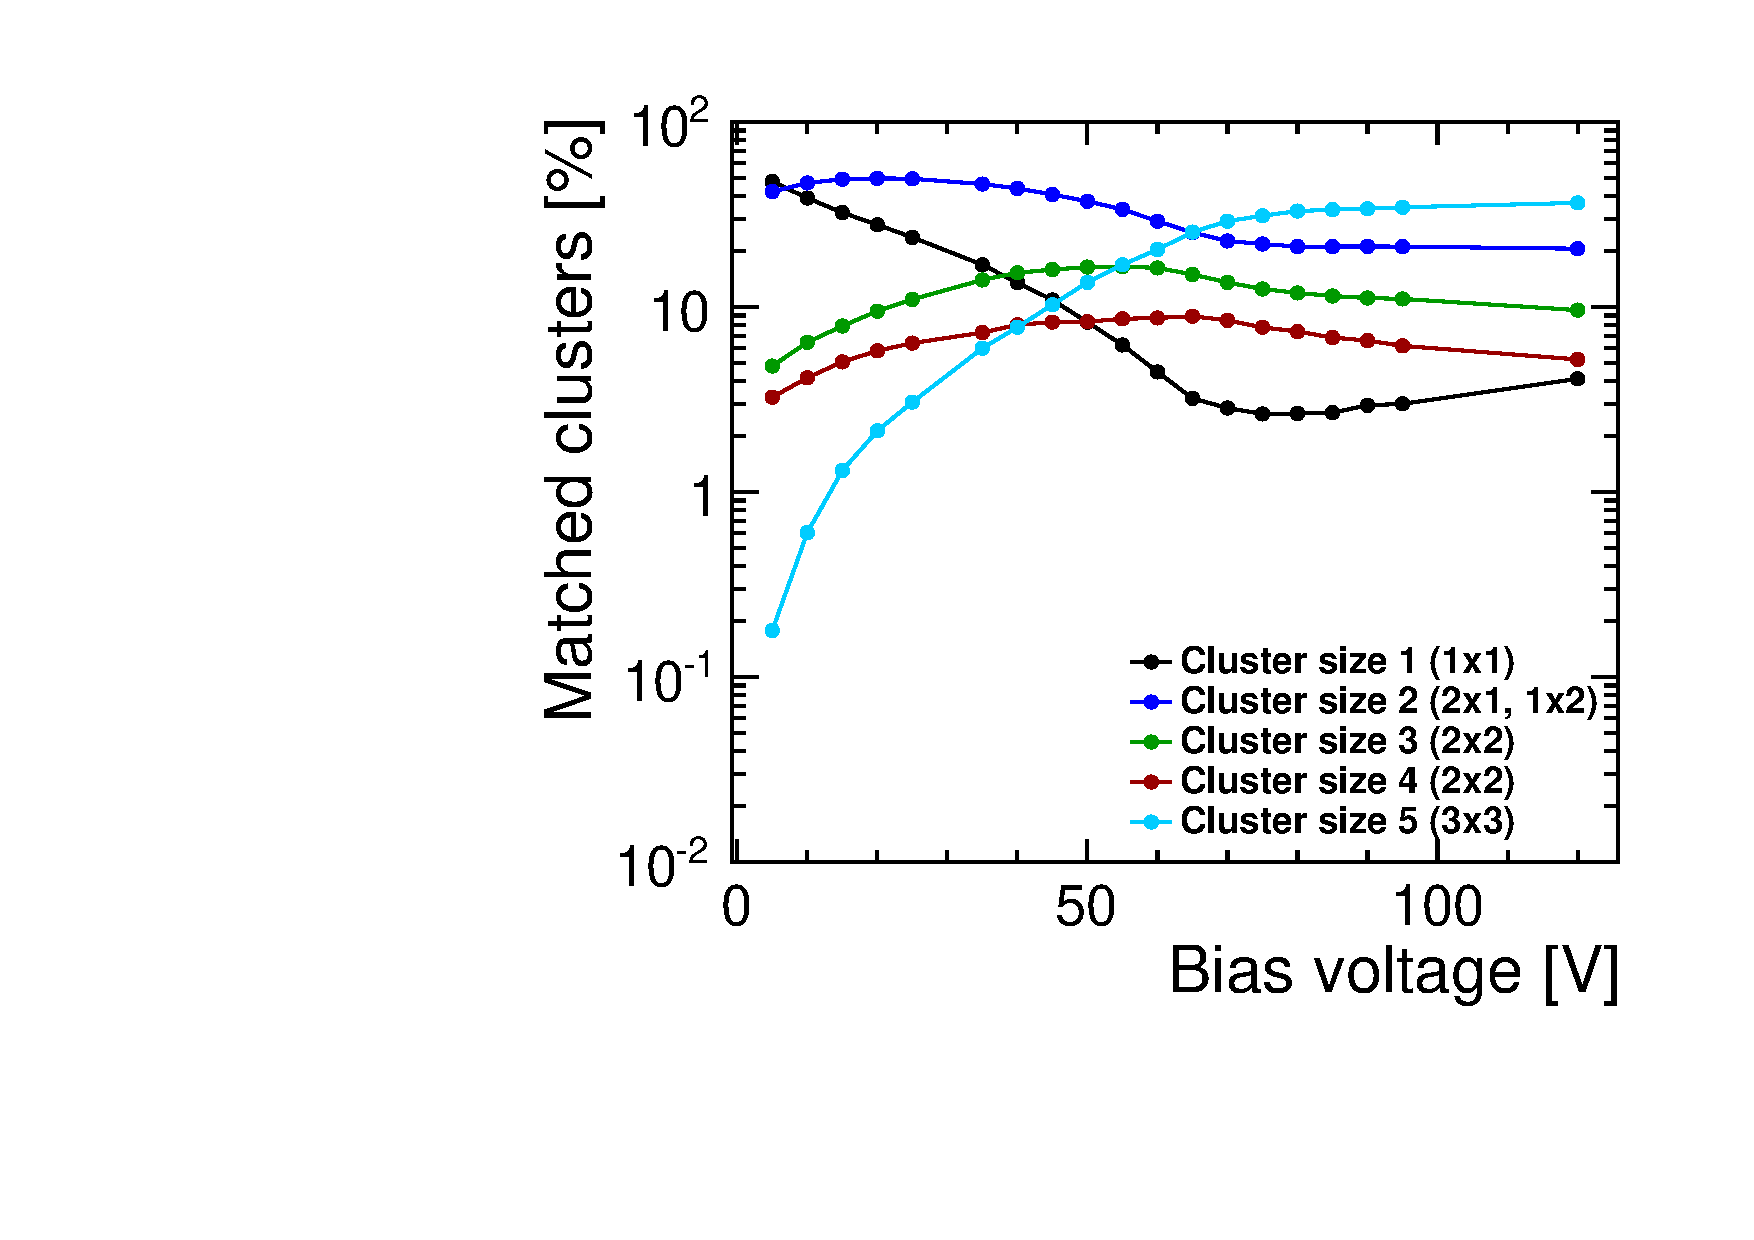
\includegraphics[width=\textwidth]{./figures/TestBeam/cluSize_biasScan_W0002_J05.pdf}
    \caption{W2\_J5}
  \end{subfigure}
  \caption{Cluster sizes vs. bias voltage.}
  \label{fig:clusterSize_vs_biasVoltage}
\end{figure}

\subsection{Cluster size vs. threshold}
\begin{figure}[htbp] \centering
  \begin{subfigure}[b]{0.33\textwidth}
    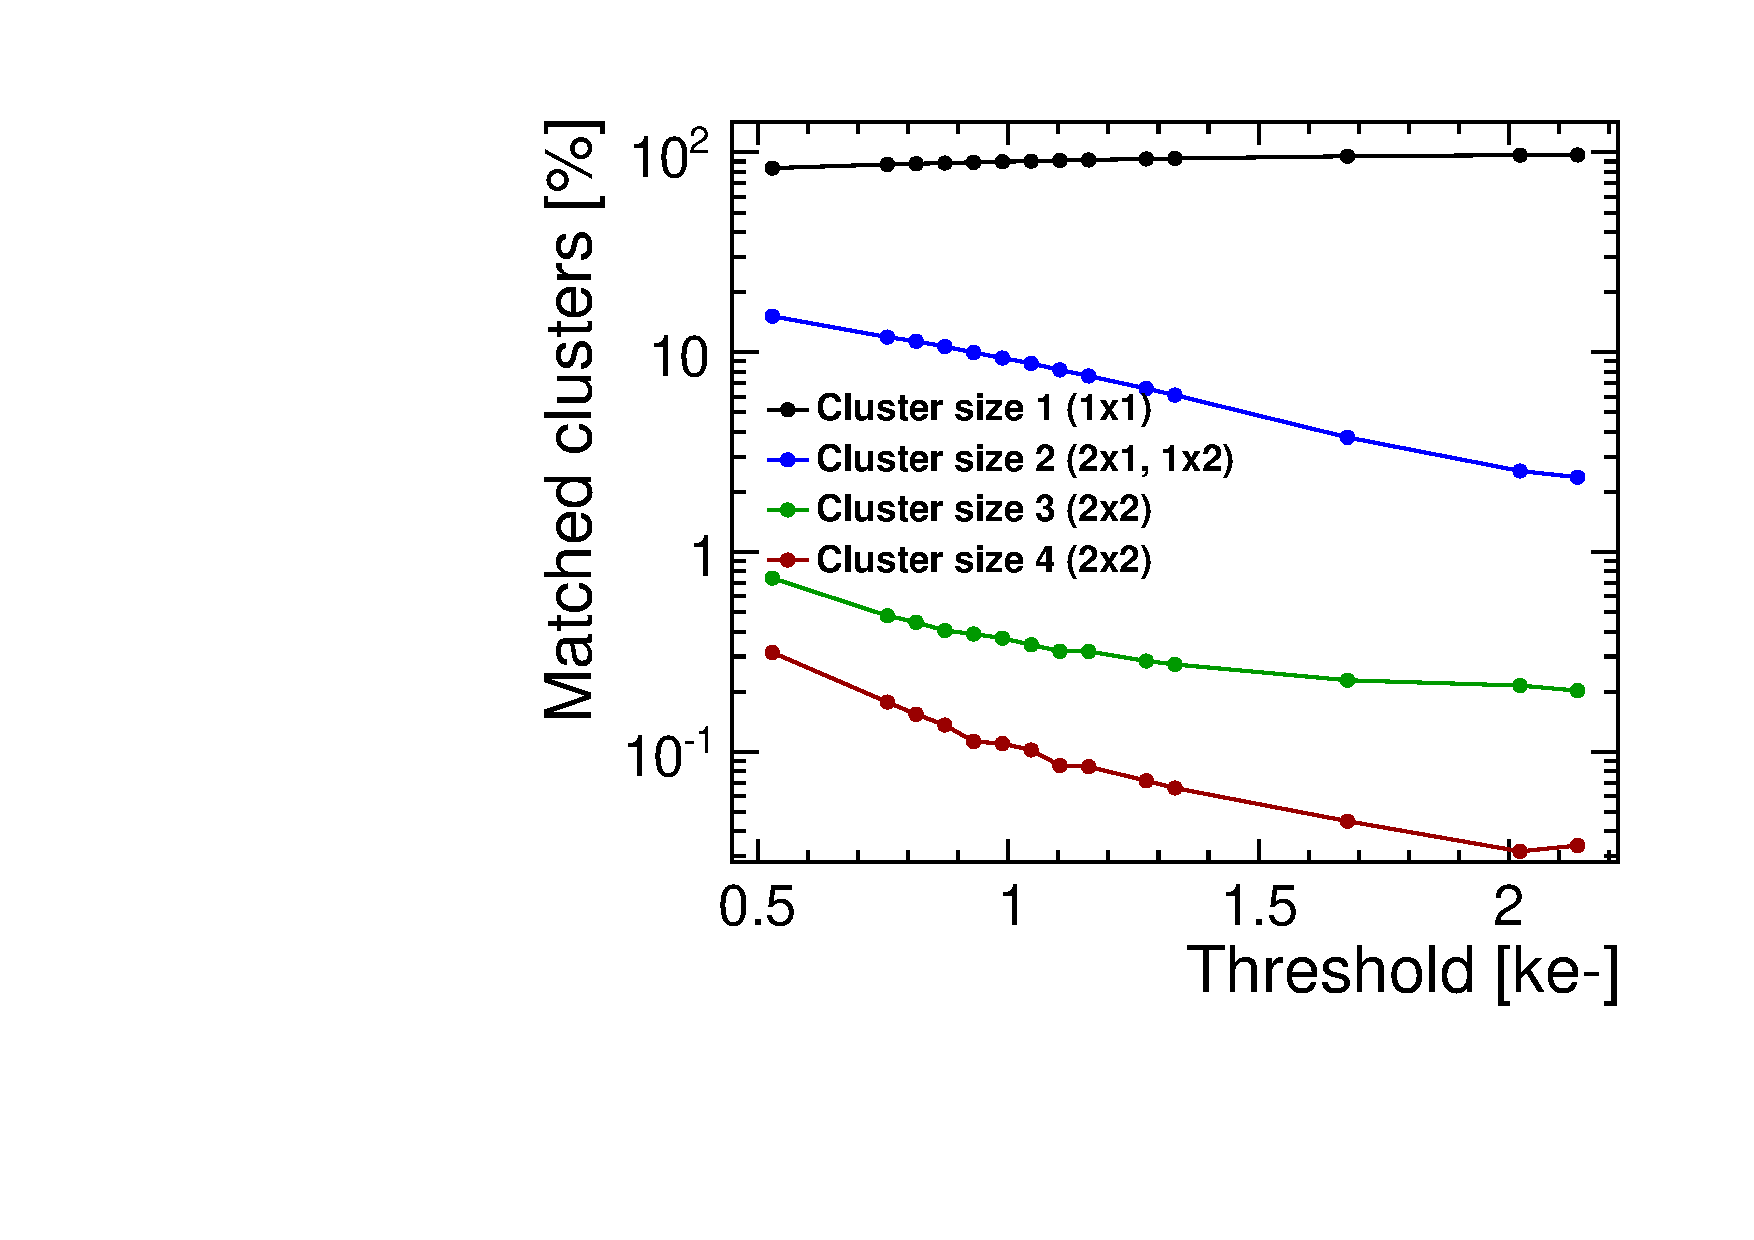
\includegraphics[width=\textwidth]{./figures/TestBeam/cluSize_THLscan_W0019_G07.pdf}
    \caption{20-NGR}
  \end{subfigure} \hfill
  \begin{subfigure}[b]{0.33\textwidth}
    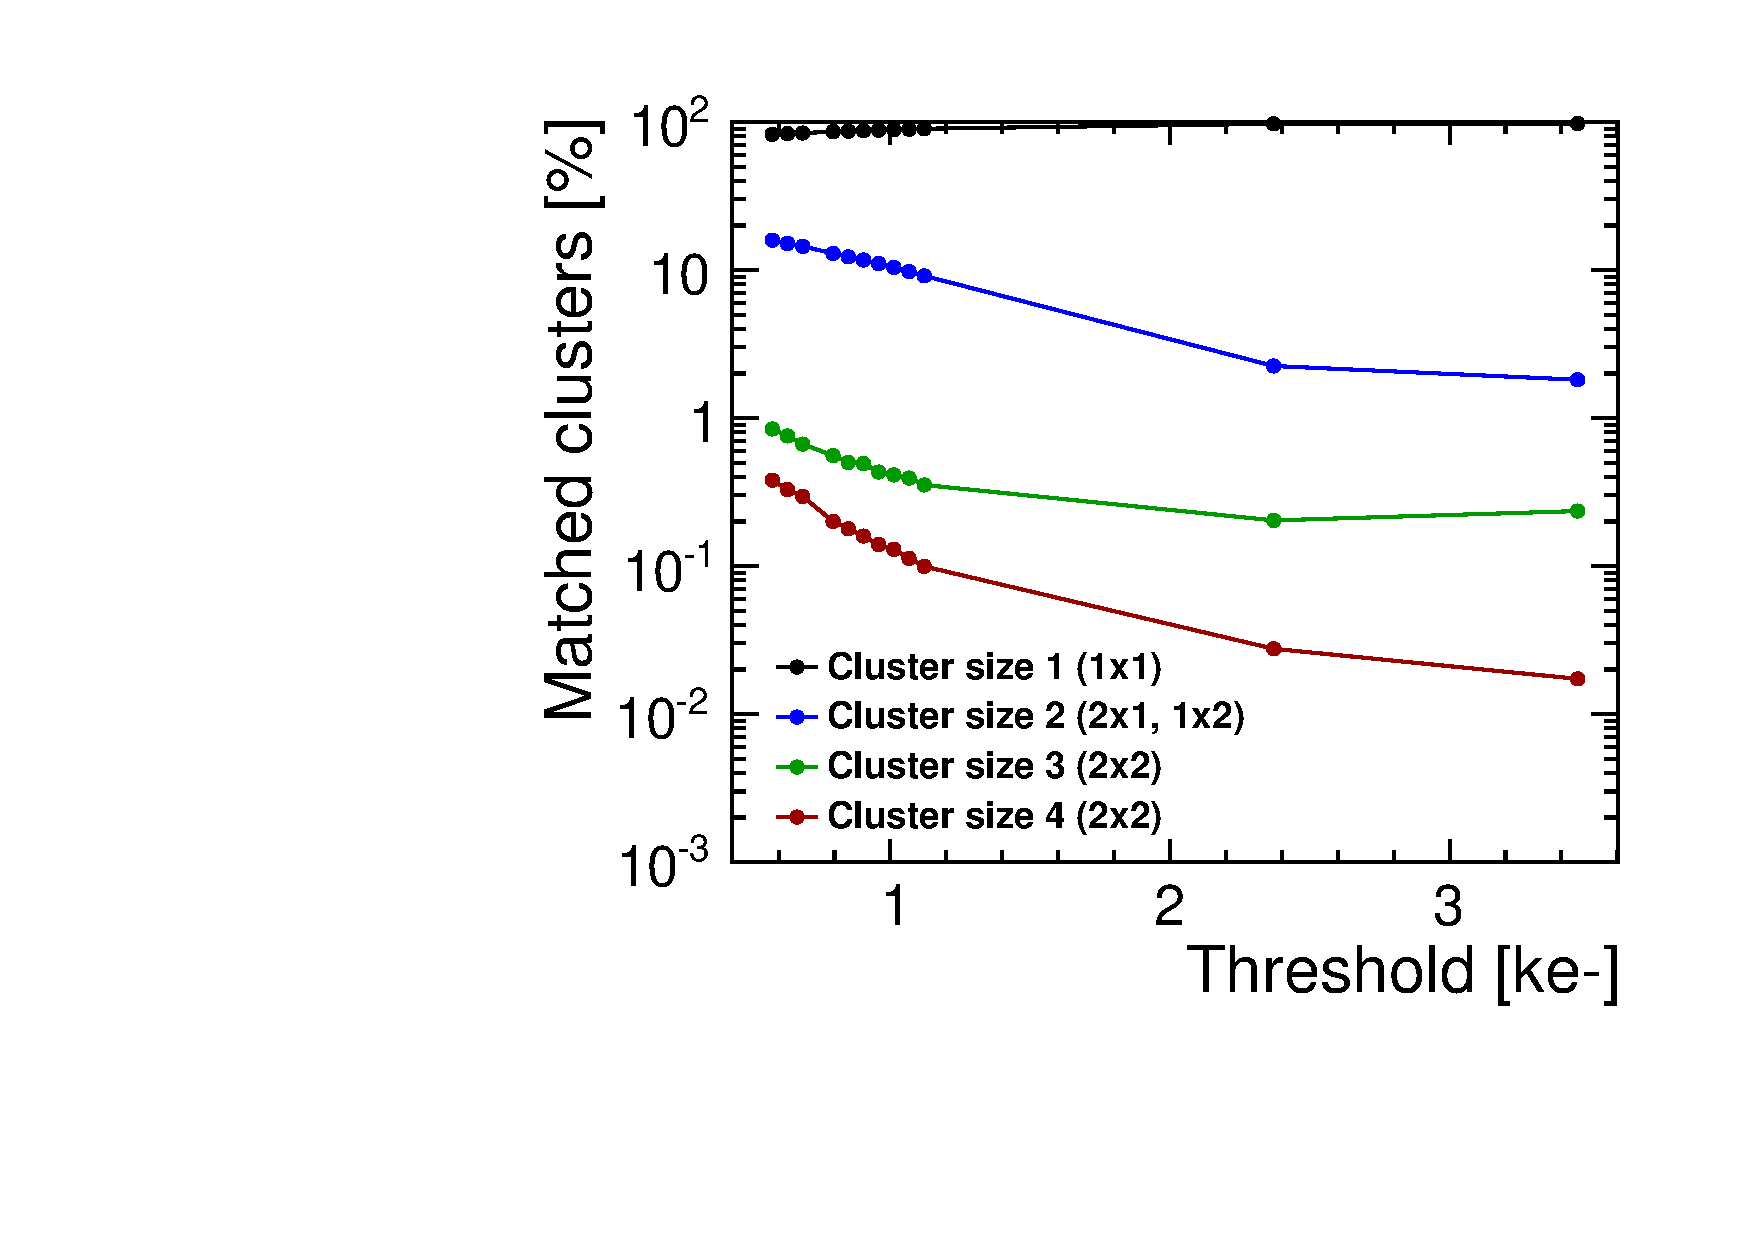
\includegraphics[width=\textwidth]{./figures/TestBeam/cluSize_THLscan_W0019_F07.pdf}
    \caption{23-FGR}
  \end{subfigure}\hfill
  \begin{subfigure}[b]{0.33\textwidth}
    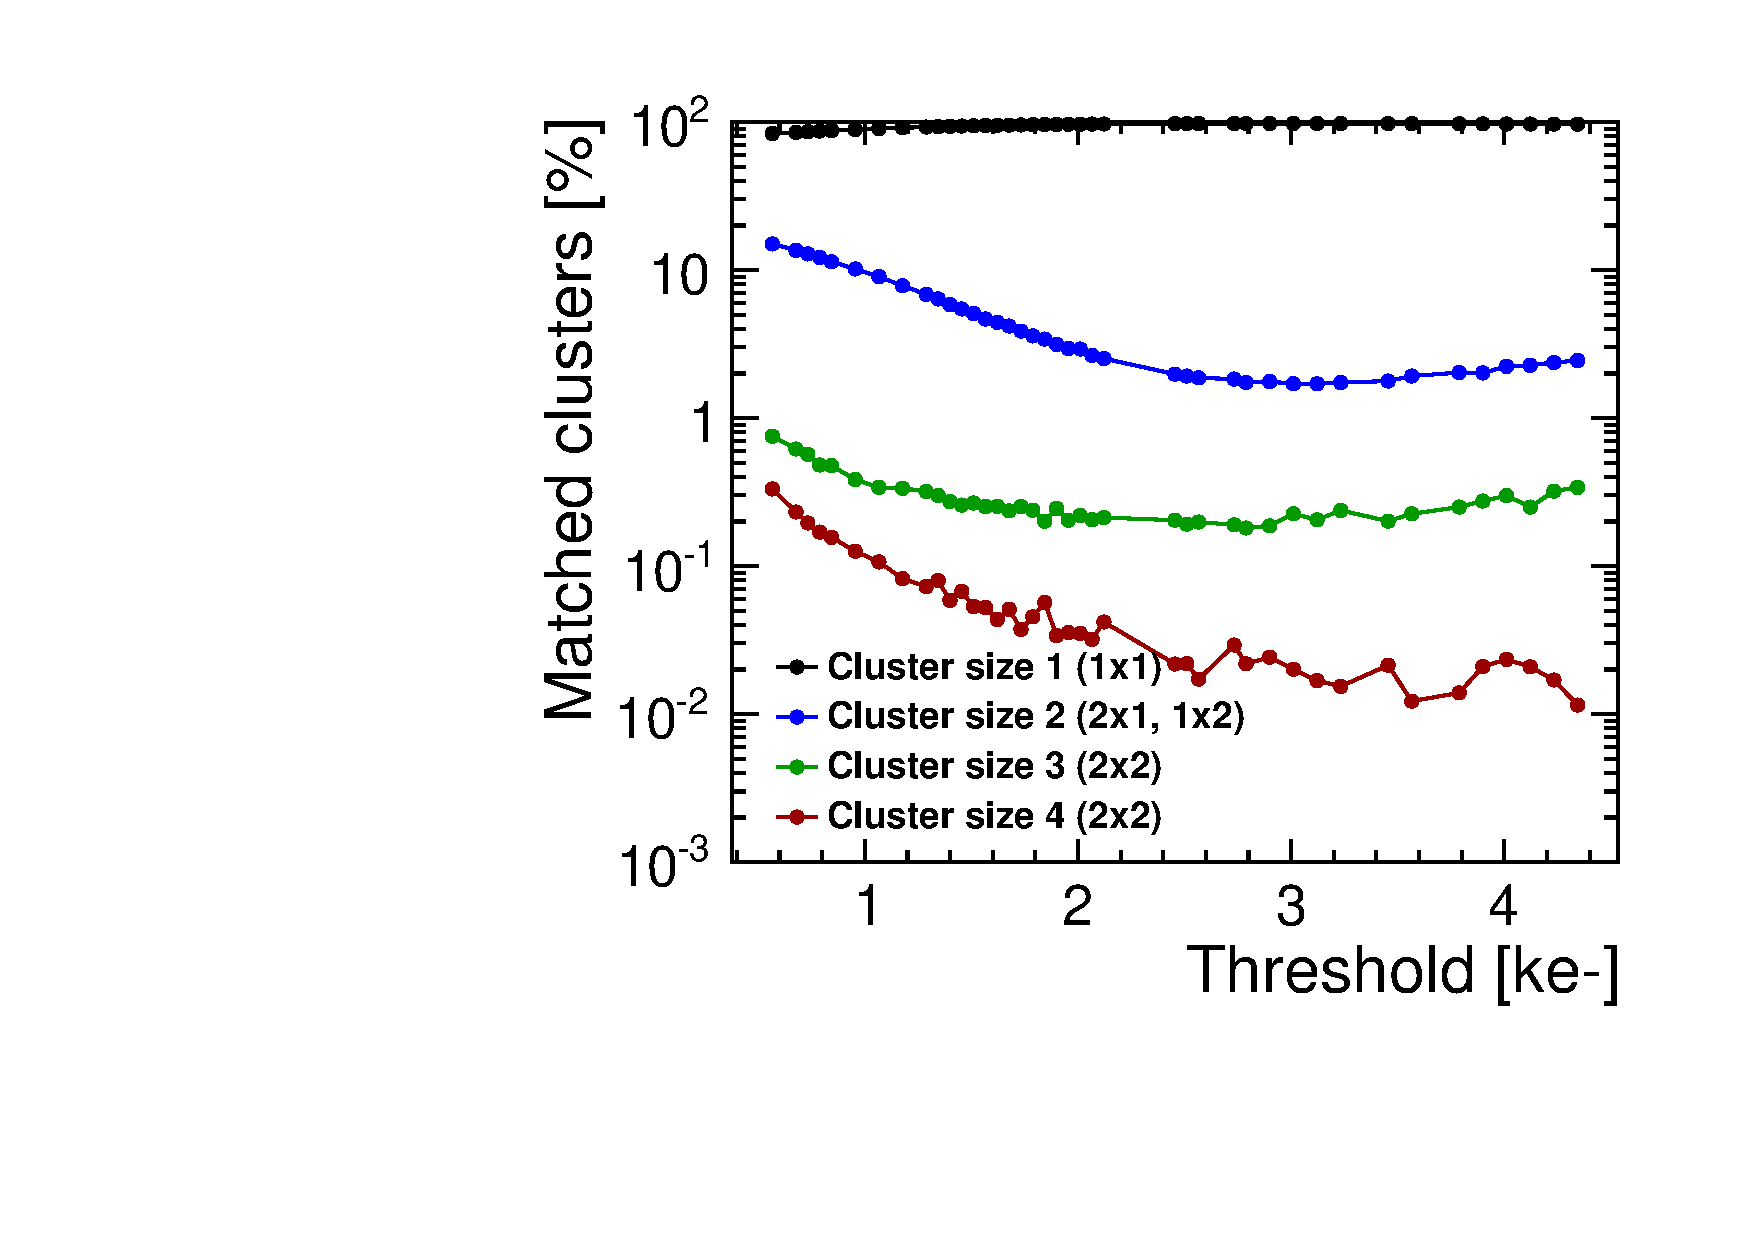
\includegraphics[width=\textwidth]{./figures/TestBeam/cluSize_THLscan_W0019_L08.pdf}
    \caption{28-GNDGR}
  \end{subfigure} \\

  \begin{subfigure}[b]{0.33\textwidth}
    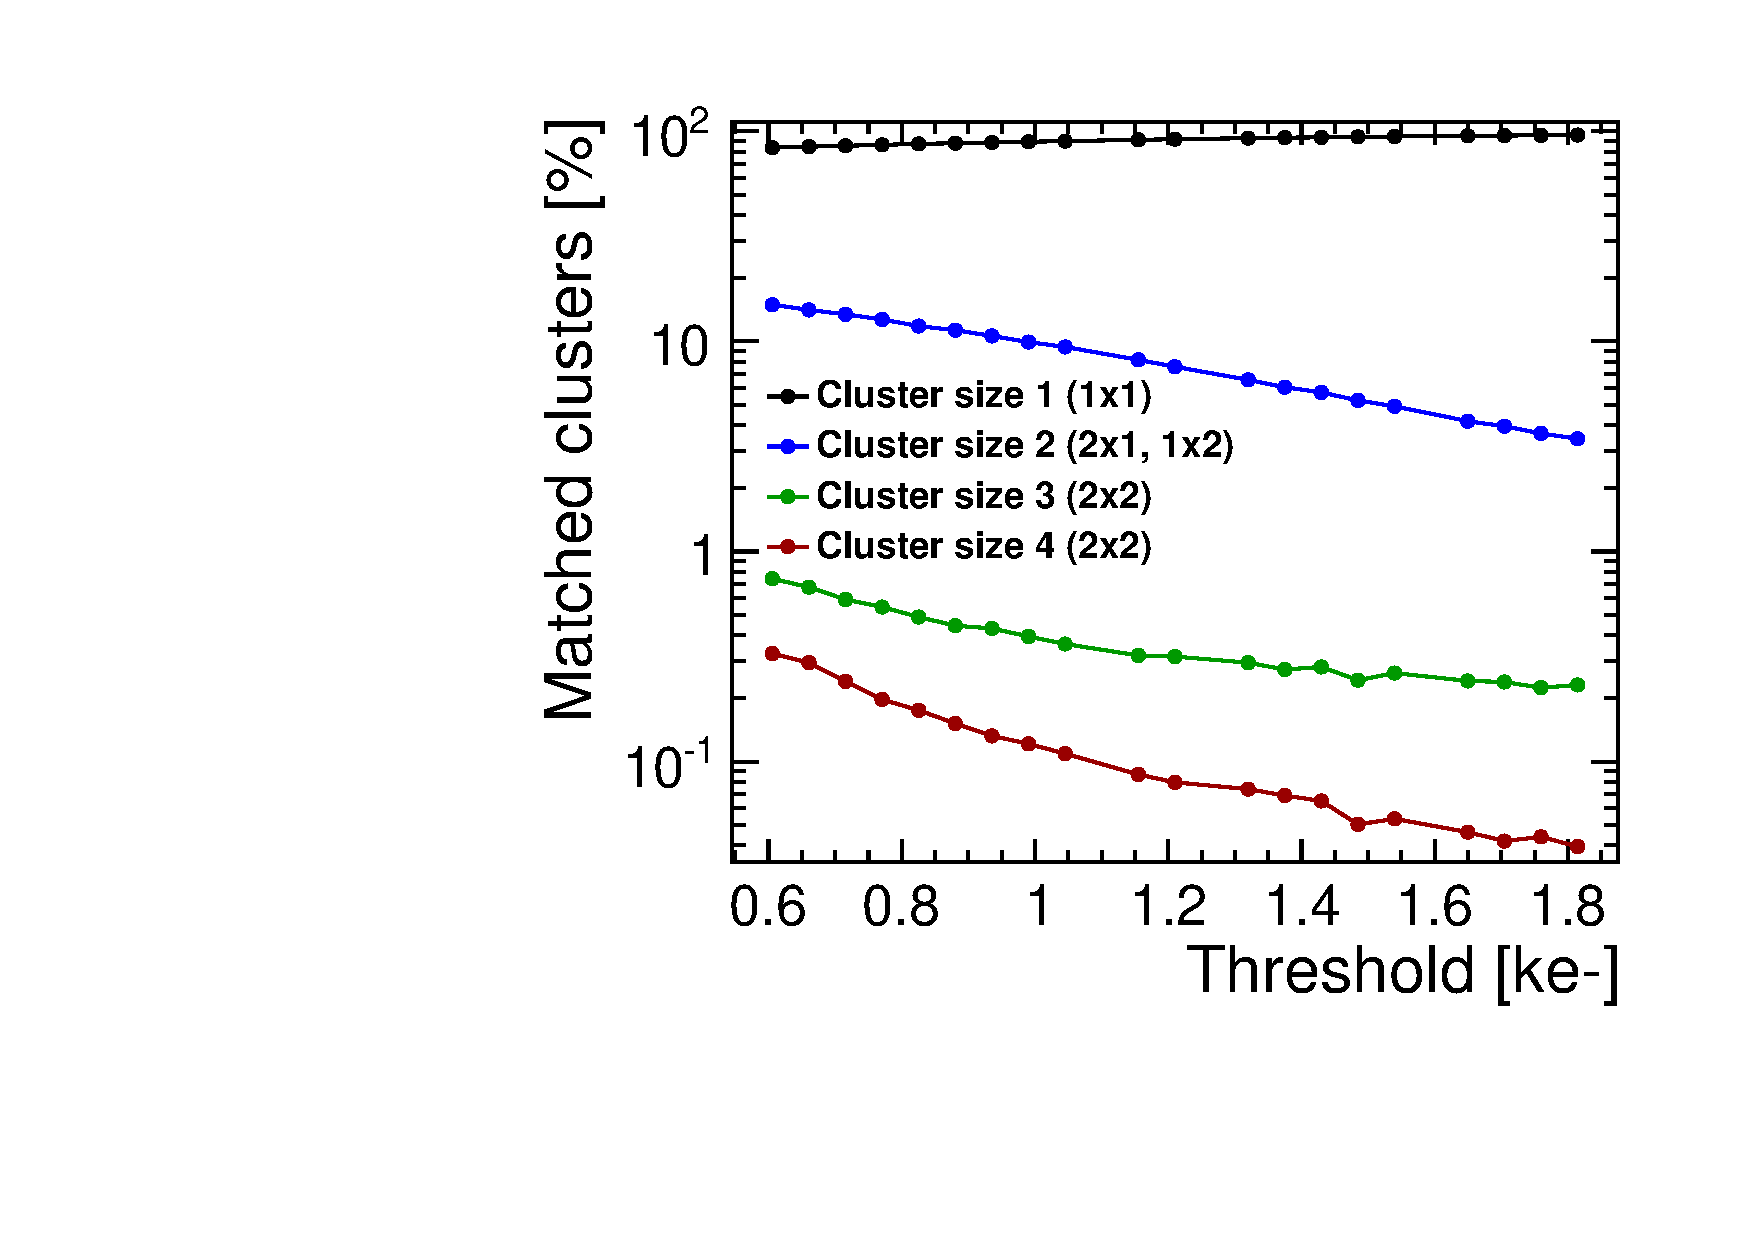
\includegraphics[width=\textwidth]{./figures/TestBeam/cluSize_THLscan_W0019_C07.pdf}
    \caption{55-GNDGR}
  \end{subfigure} \hfill
  \begin{subfigure}[b]{0.33\textwidth}
    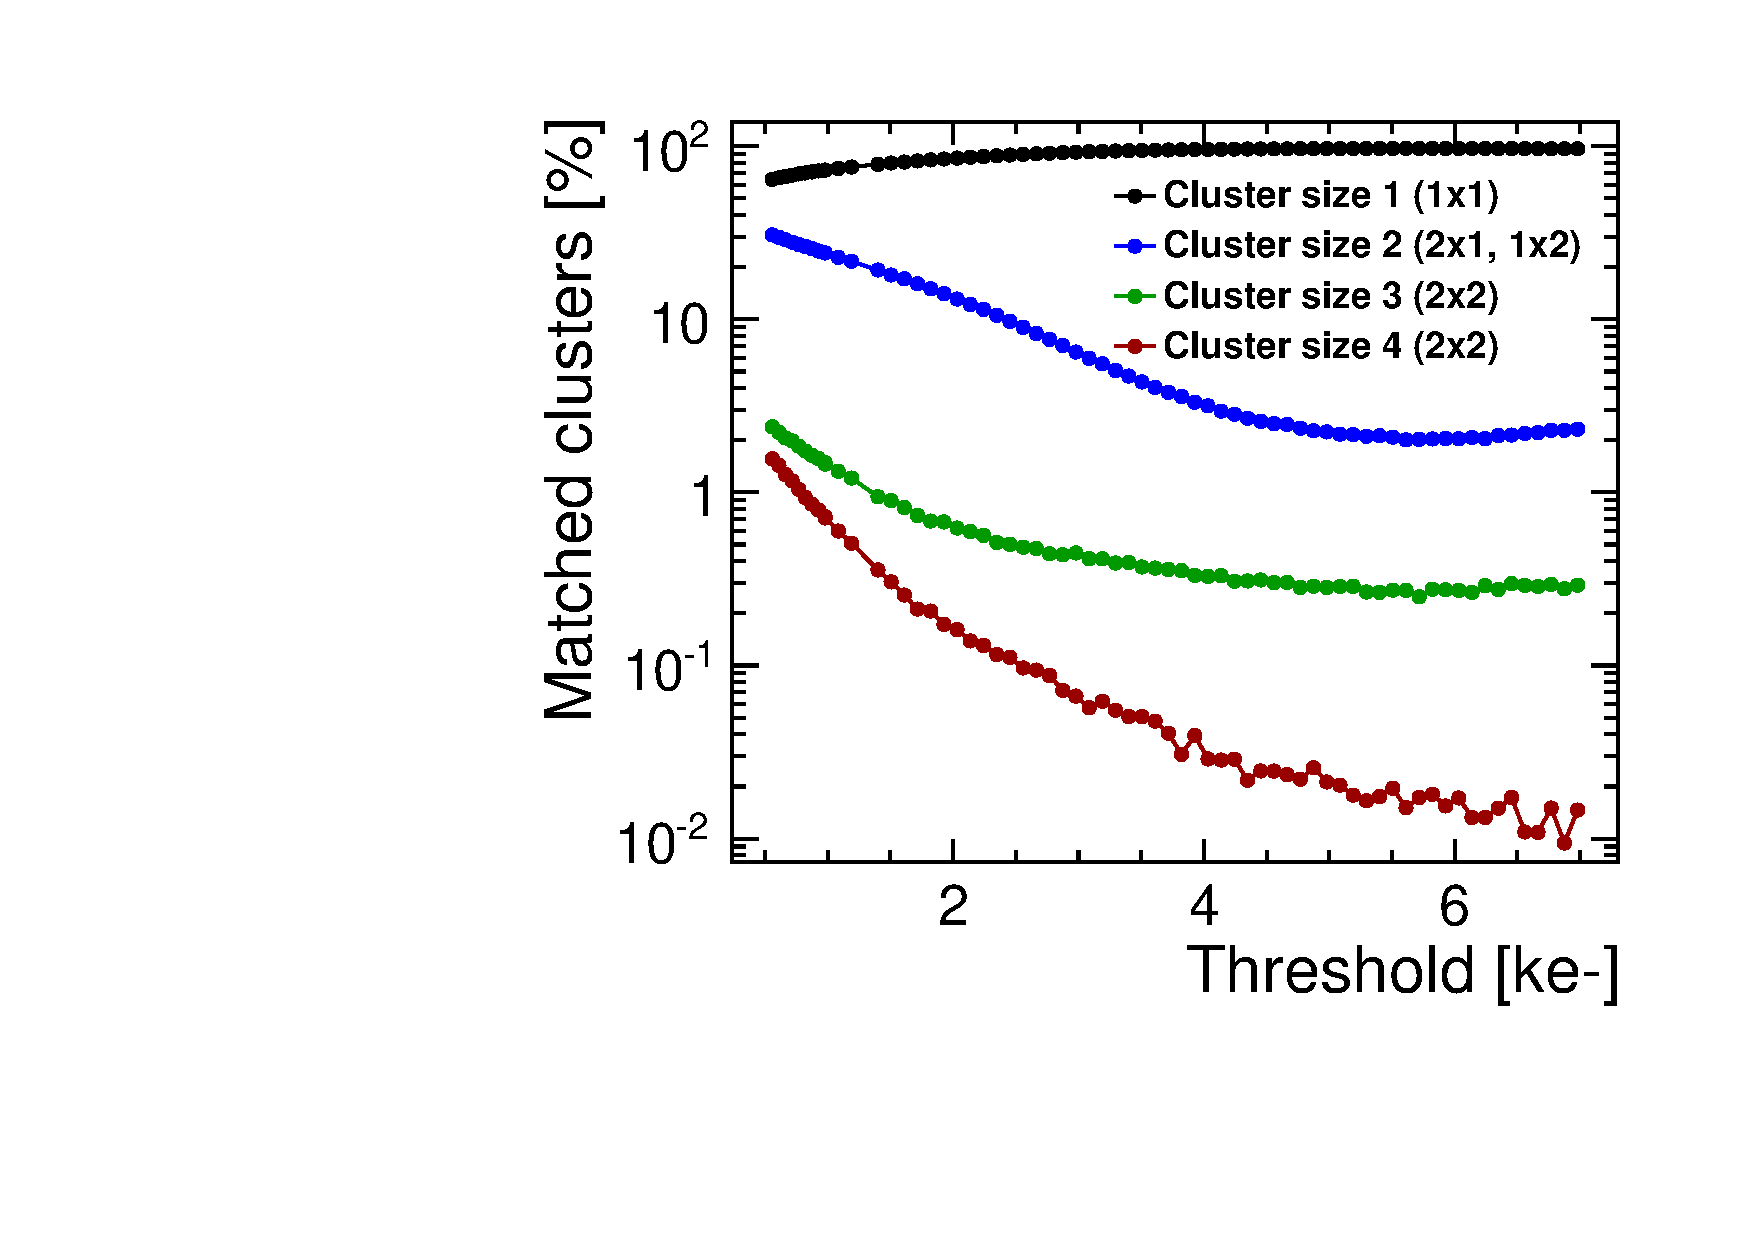
\includegraphics[width=\textwidth]{./figures/TestBeam/cluSize_THLscan_W0005_E02.pdf}
    \caption{55-GND-GR-100}
  \end{subfigure}\hfill
  \begin{subfigure}[b]{0.33\textwidth}
    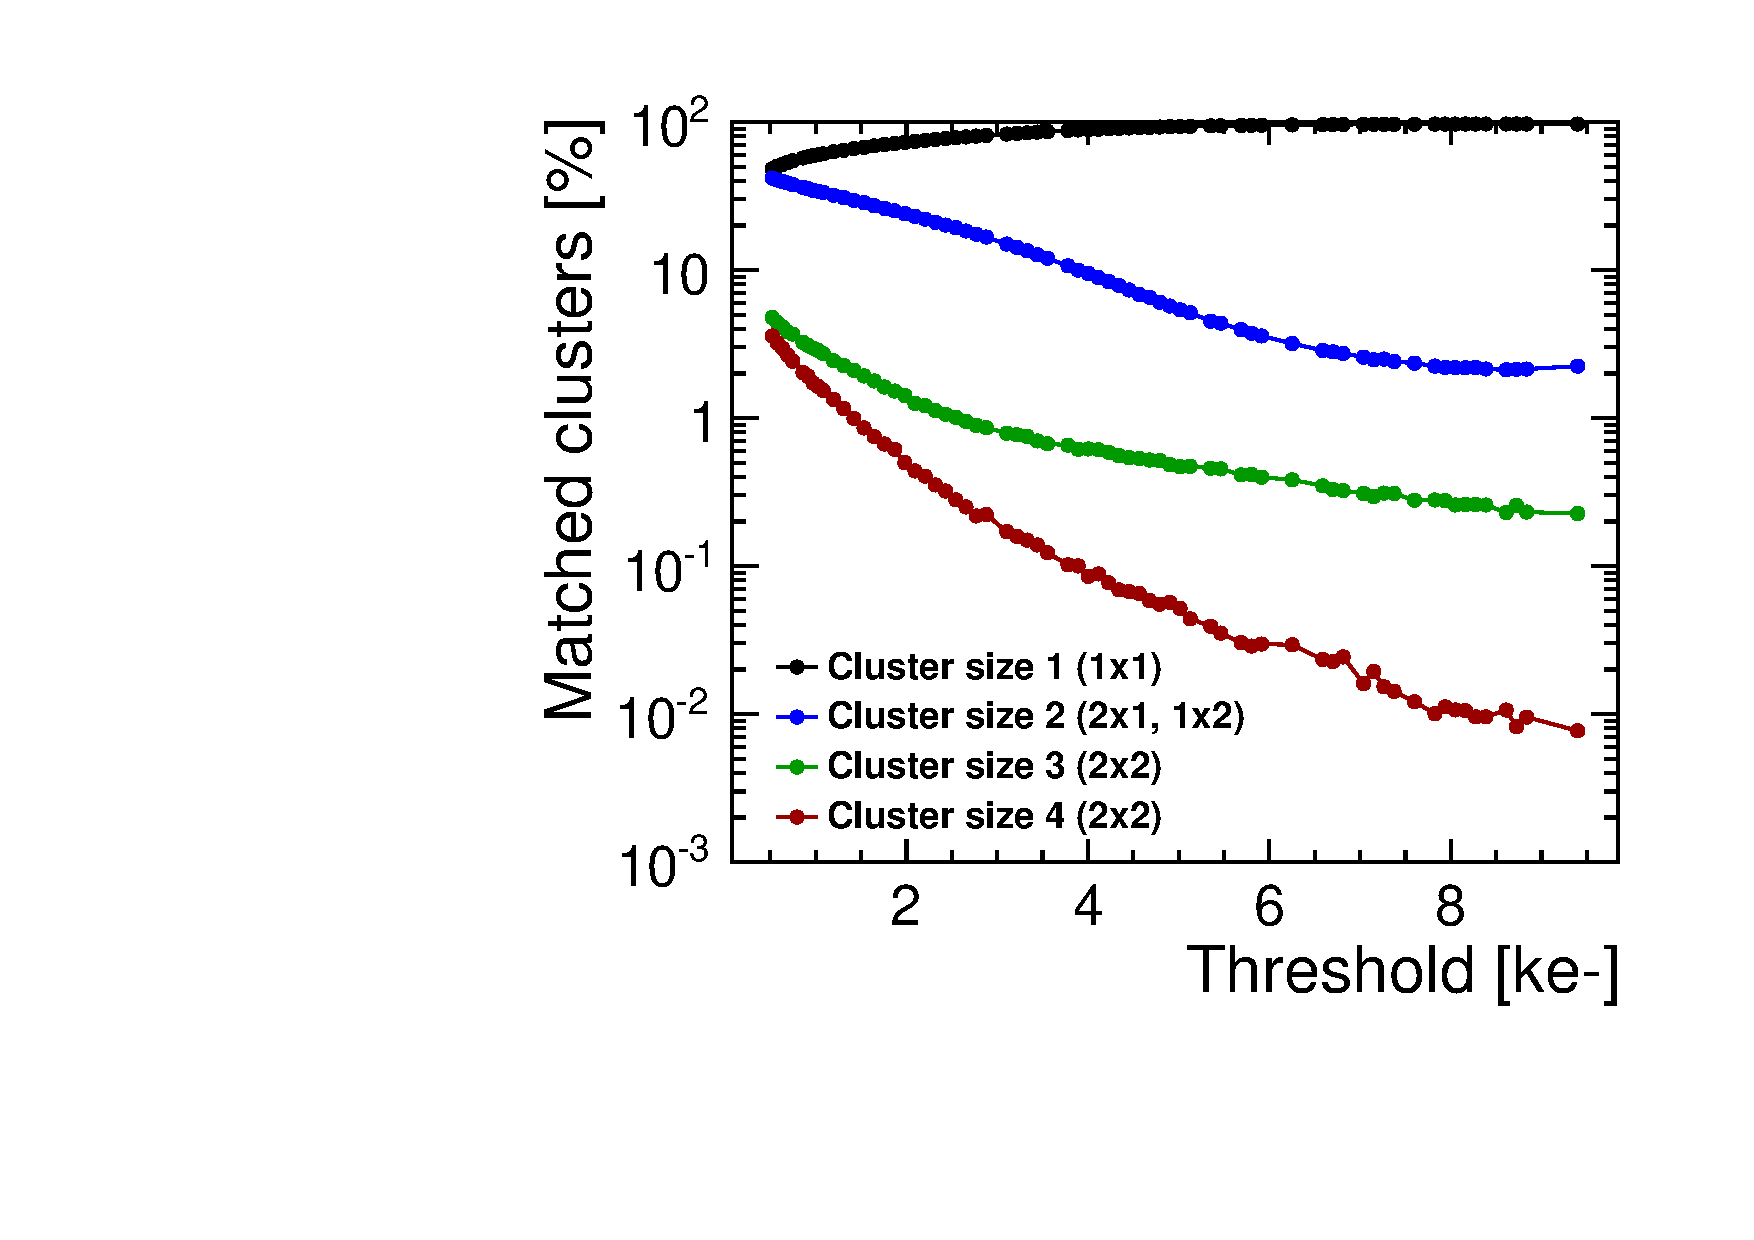
\includegraphics[width=\textwidth]{./figures/TestBeam/cluSize_THLscan_W0005_F01.pdf}
    \caption{55-GND-GR-150}
  \end{subfigure}\\
  \begin{subfigure}[b]{0.33\textwidth}
    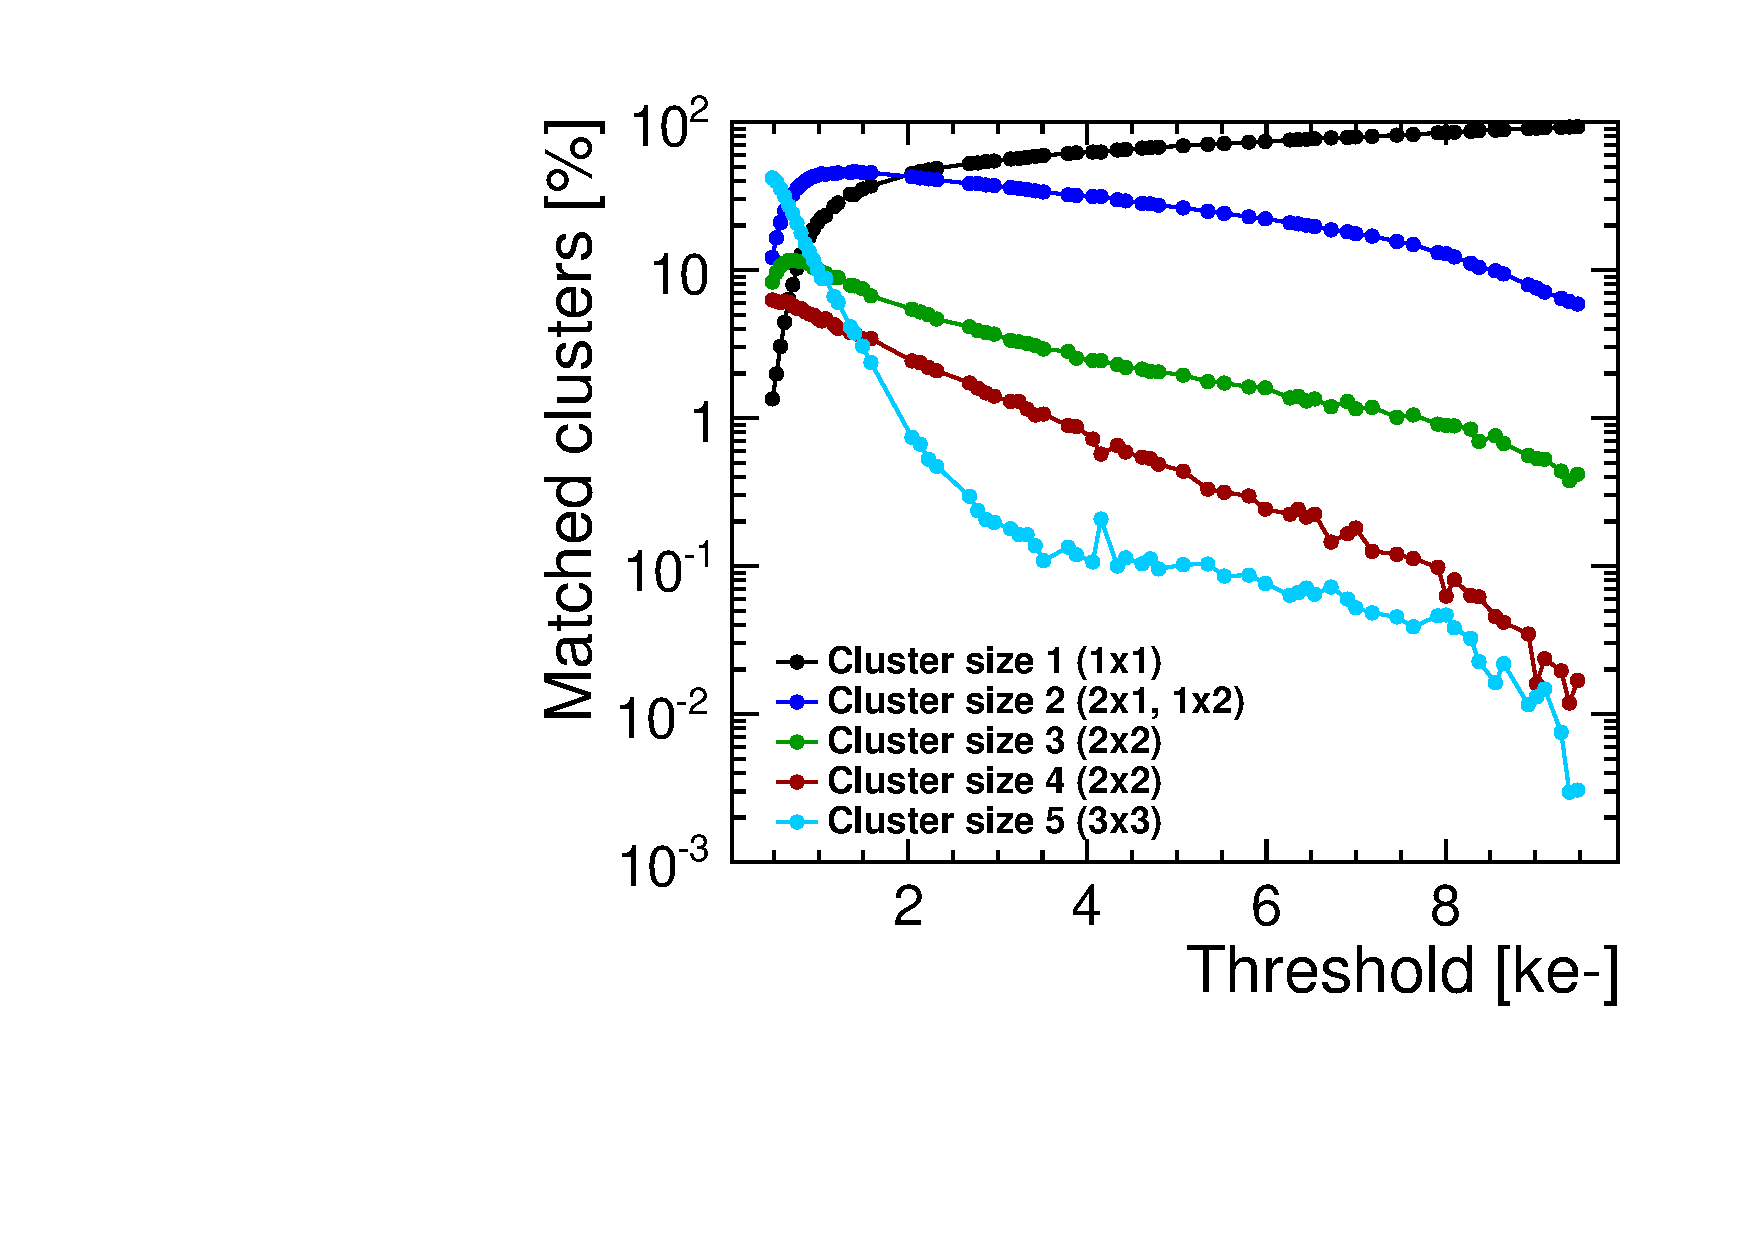
\includegraphics[width=\textwidth]{./figures/TestBeam/cluSize_THLscan_W0002_J05.pdf}
    \caption{W2\_J5}
  \end{subfigure}
  \caption{Cluster sizes vs. threshold.}
  \label{fig:clusterSize_vs_THLscan}
\end{figure}
\newpage
%% --------------------------------------------- %%
\section{Residuals}
\subsection{Residuals vs. bias voltage}
\begin{figure}[htbp] \centering
  \begin{subfigure}[b]{0.33\textwidth}
    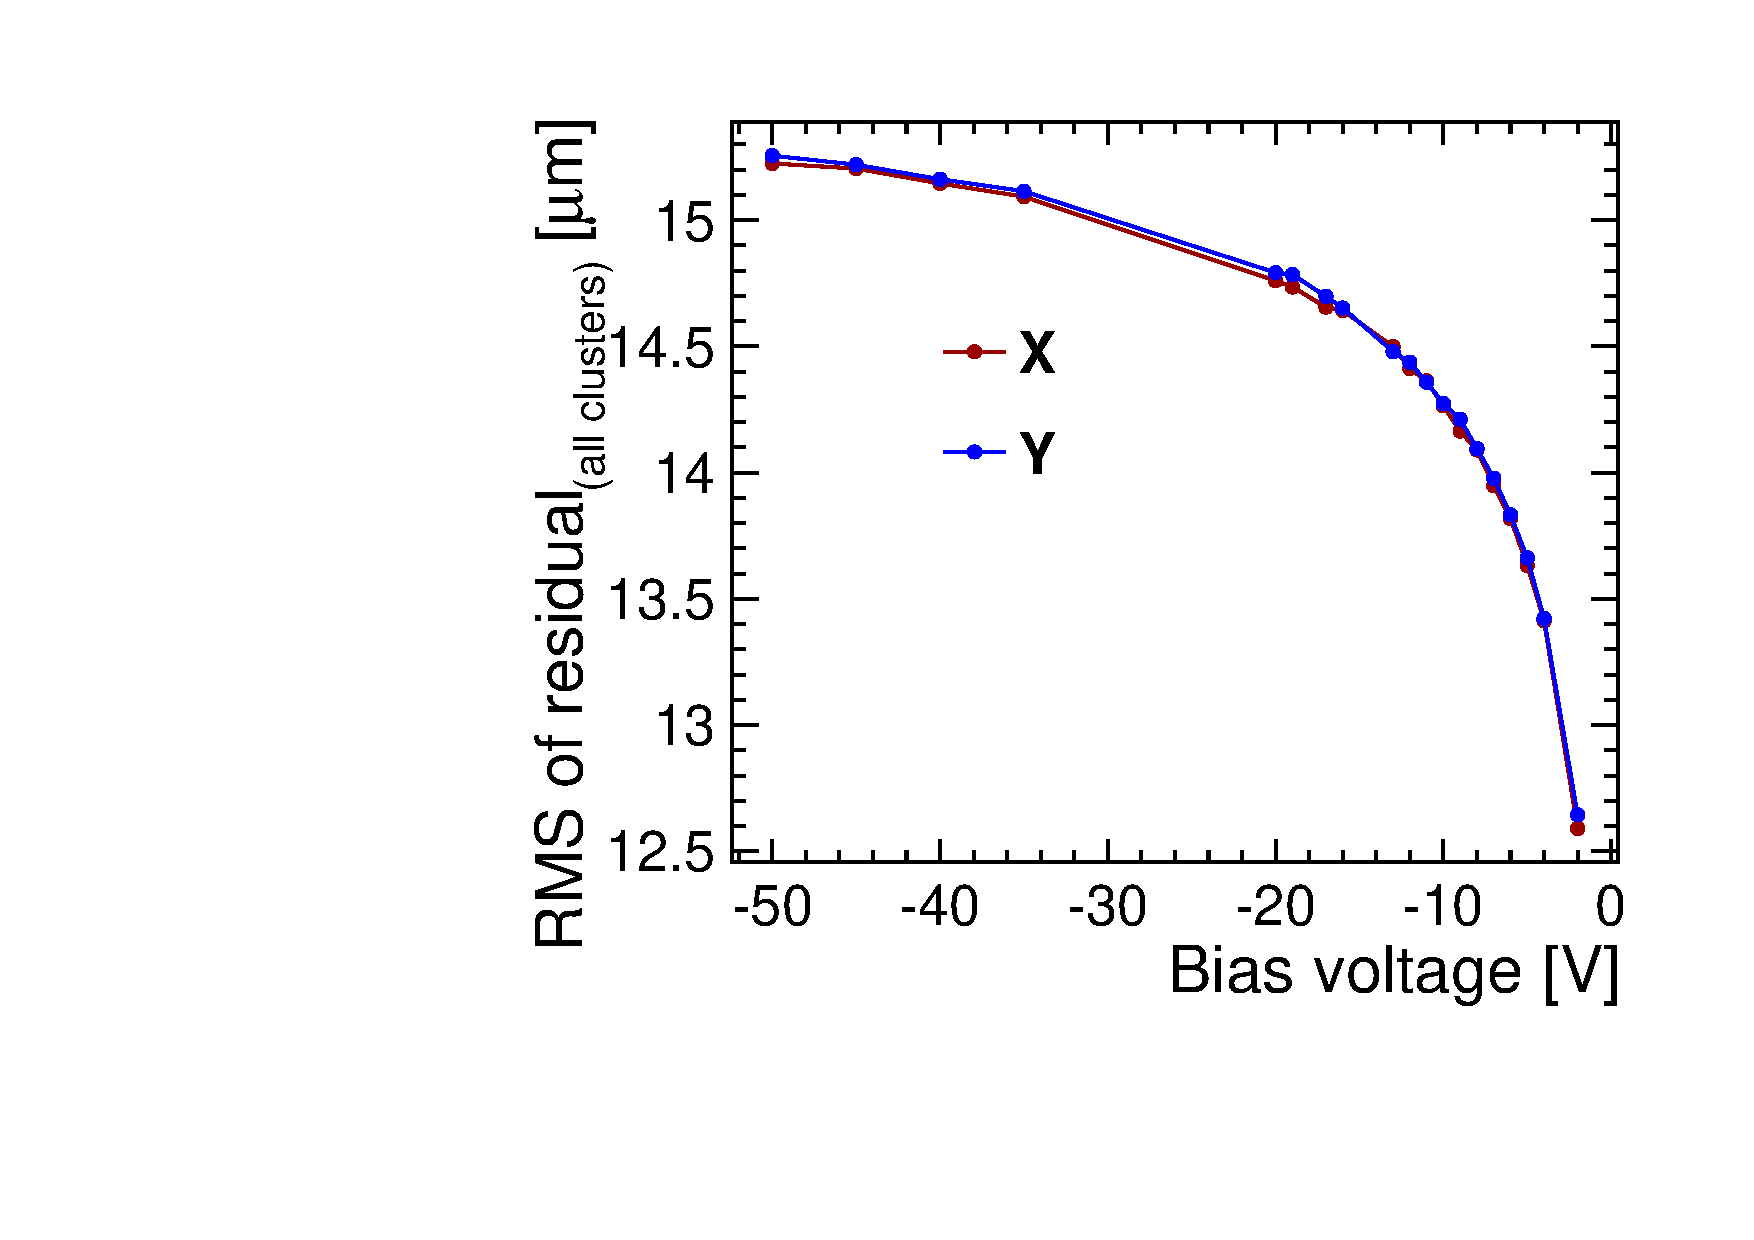
\includegraphics[width=\textwidth]{./figures/TestBeam/W19_G7_Residual_vs_bias.pdf}
    \caption{20-NGR}
  \end{subfigure} \hfill
  \begin{subfigure}[b]{0.33\textwidth}
    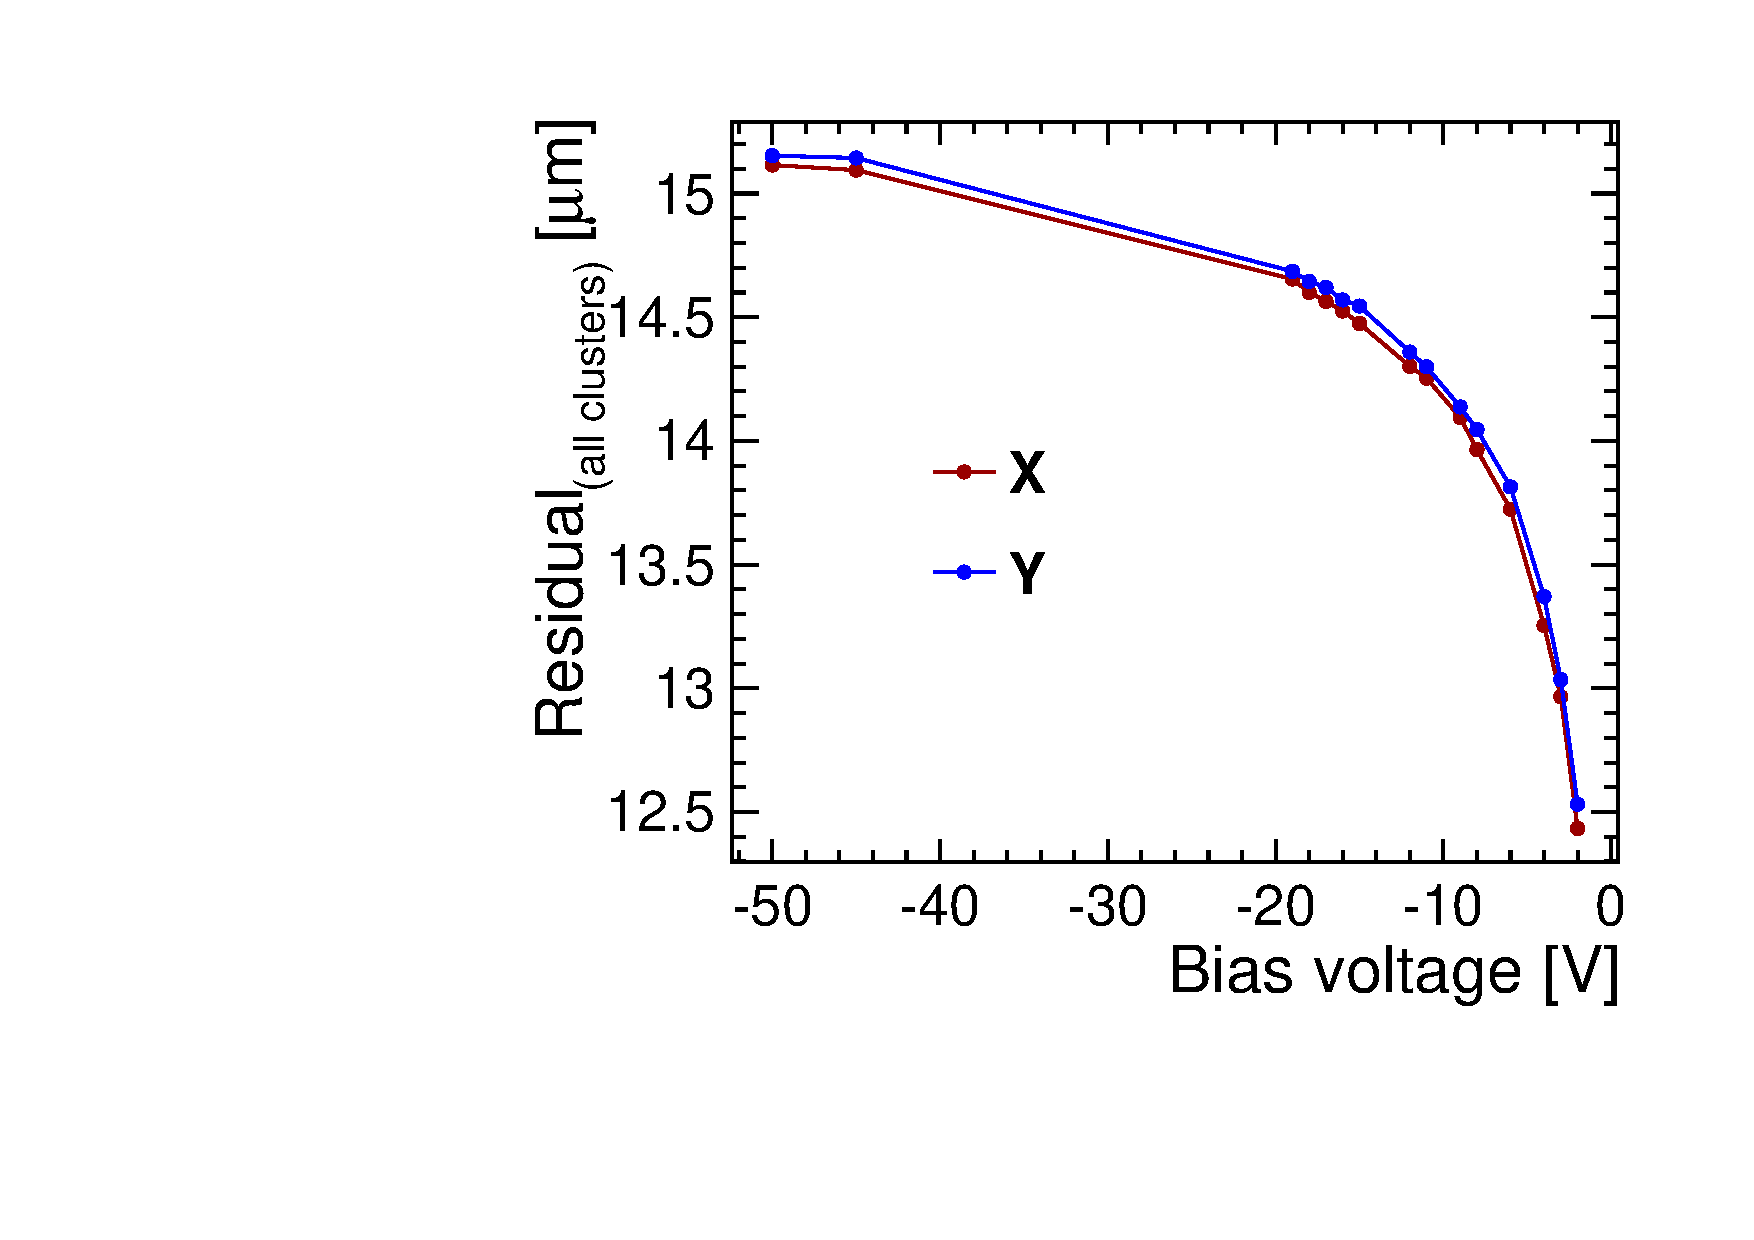
\includegraphics[width=\textwidth]{./figures/TestBeam/W19_F7_Residual_vs_bias.pdf}
    \caption{23-FGR}
  \end{subfigure}\hfill
  \begin{subfigure}[b]{0.33\textwidth}
    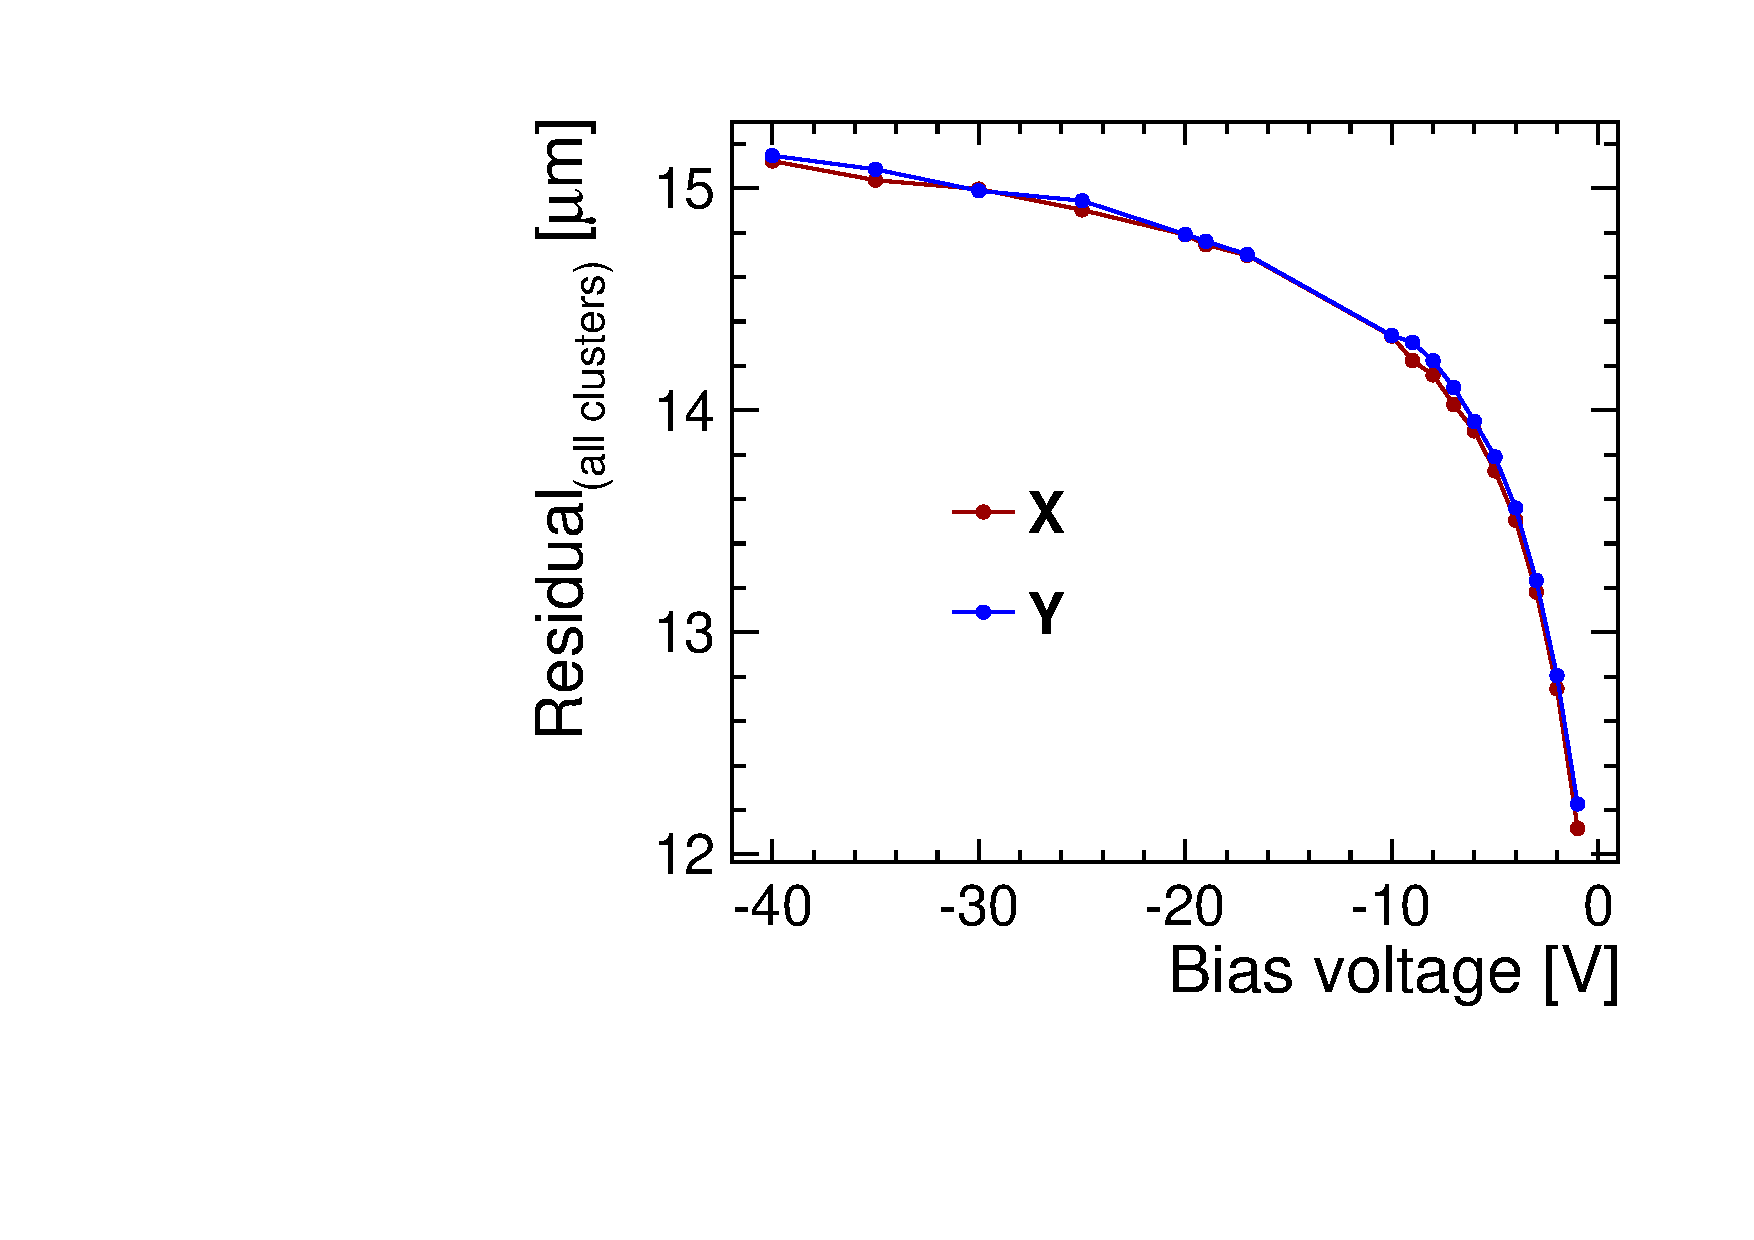
\includegraphics[width=\textwidth]{./figures/TestBeam/W19_L8_Residual_vs_bias.pdf}
    \caption{28-GNDGR}
  \end{subfigure} \\

  \begin{subfigure}[b]{0.33\textwidth}
    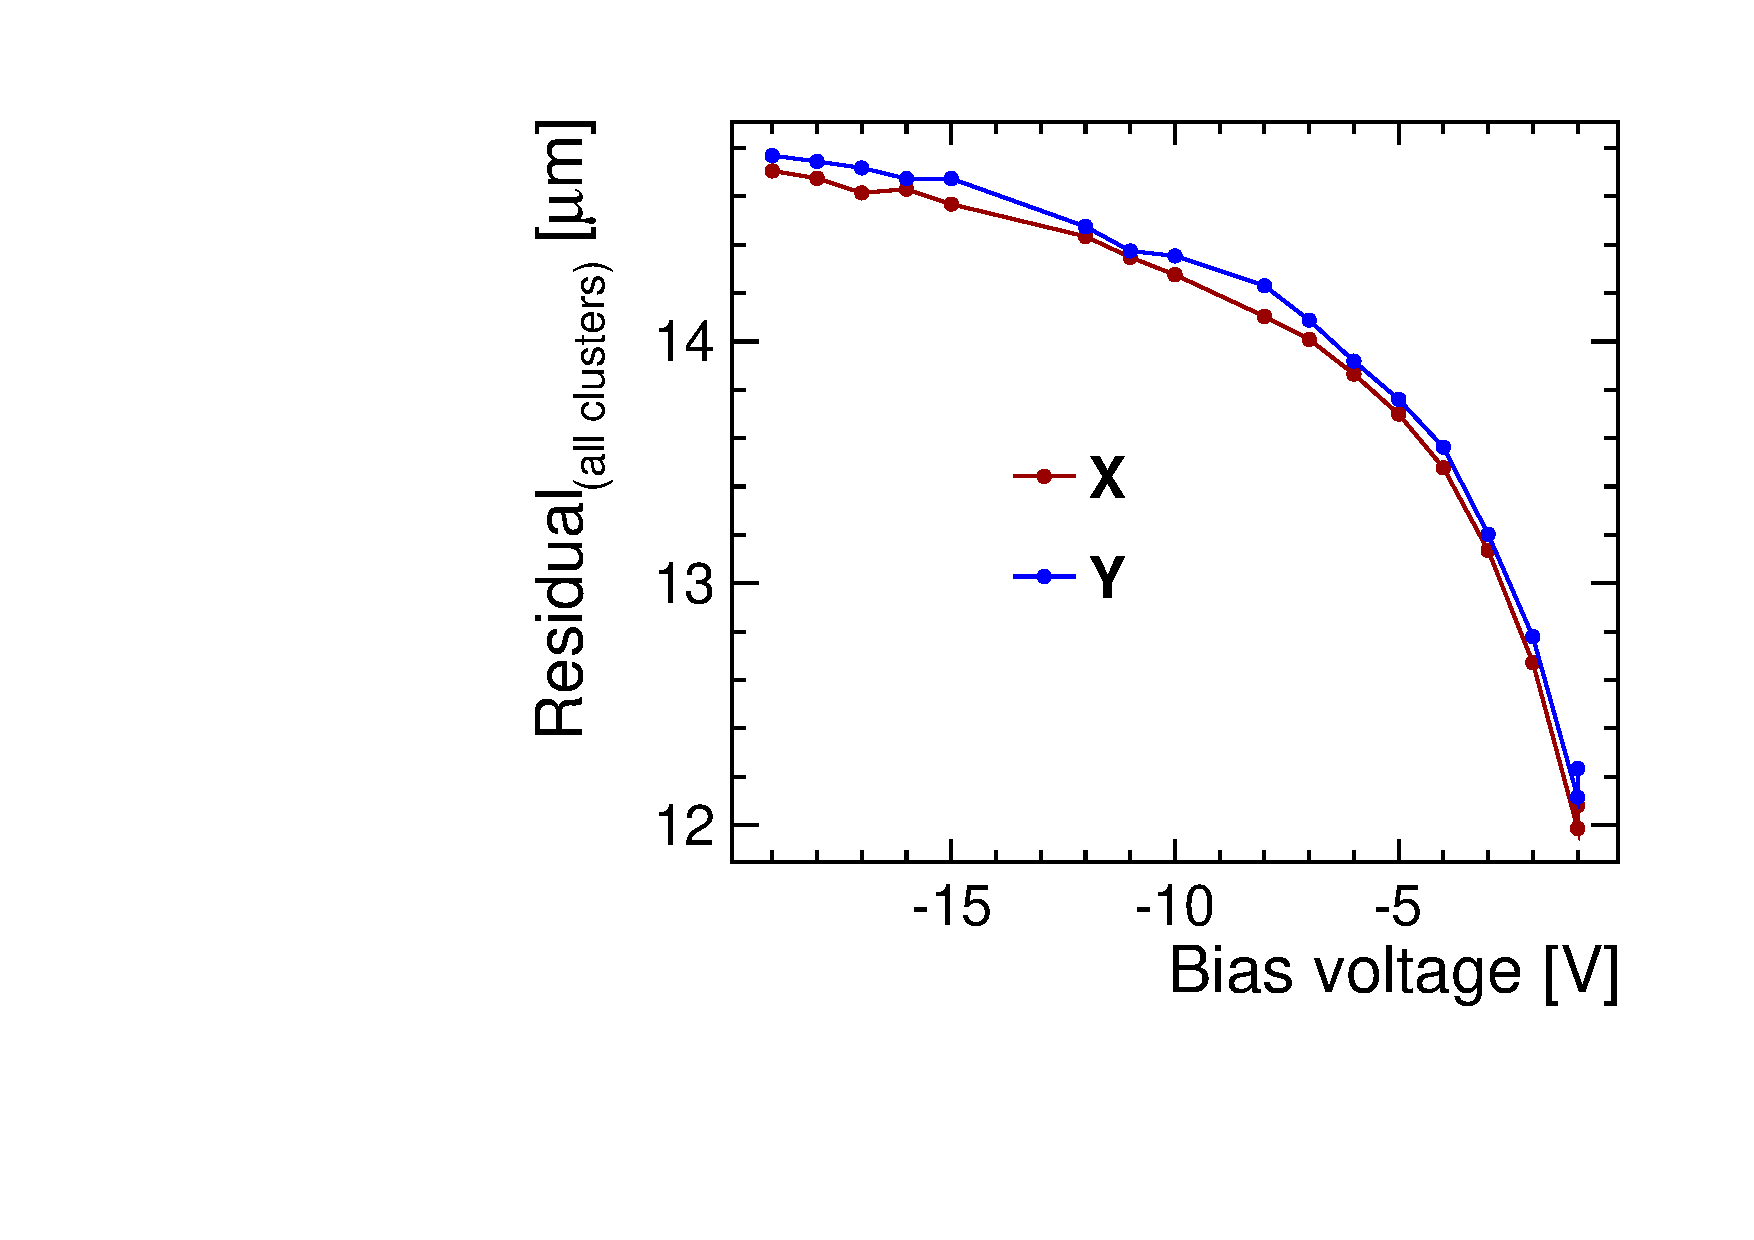
\includegraphics[width=\textwidth]{./figures/TestBeam/W19_C7_Residual_vs_bias.pdf}
    \caption{55-GNDGR}
  \end{subfigure} \hfill
  \begin{subfigure}[b]{0.33\textwidth}
    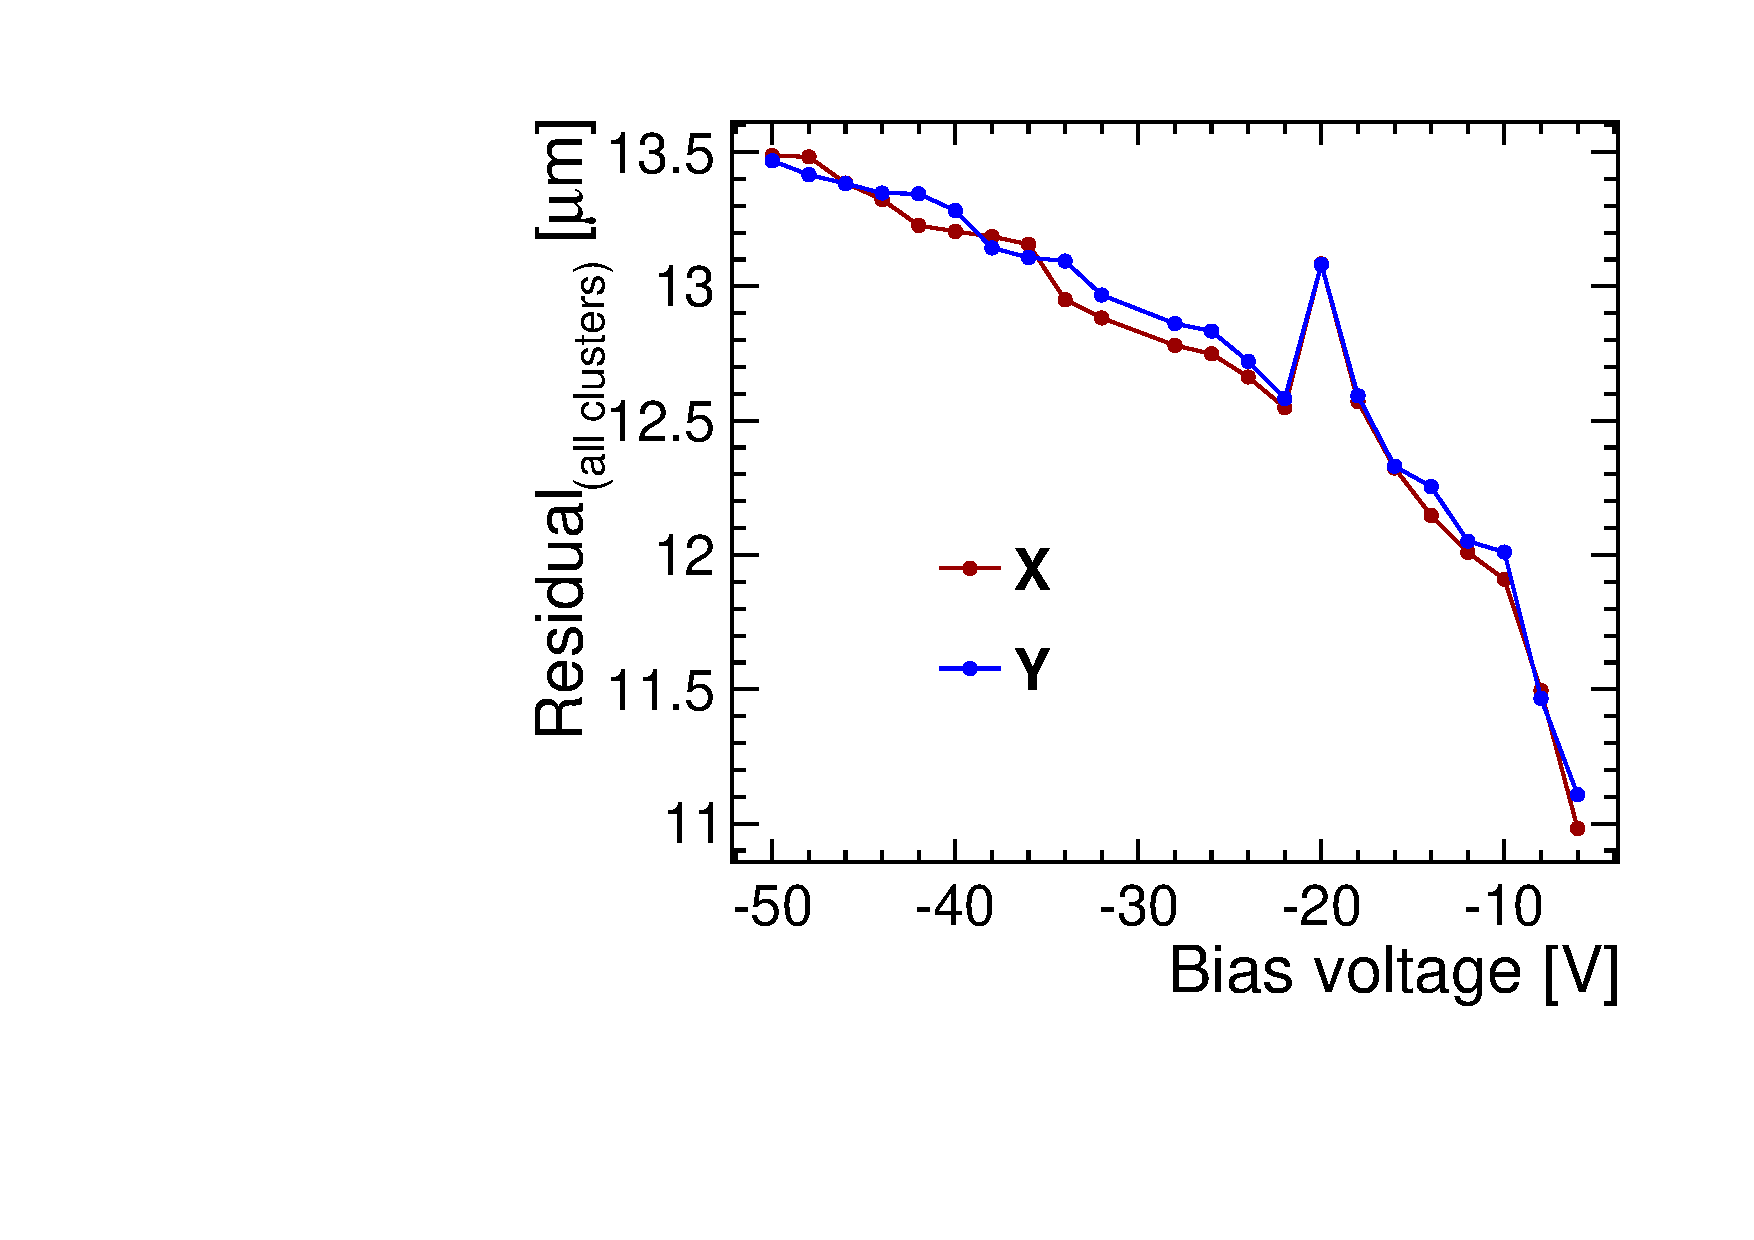
\includegraphics[width=\textwidth]{./figures/TestBeam/W5_E2_Residual_vs_bias.pdf}
    \caption{55-GND-GR-100}
  \end{subfigure}\hfill
  \begin{subfigure}[b]{0.33\textwidth}
    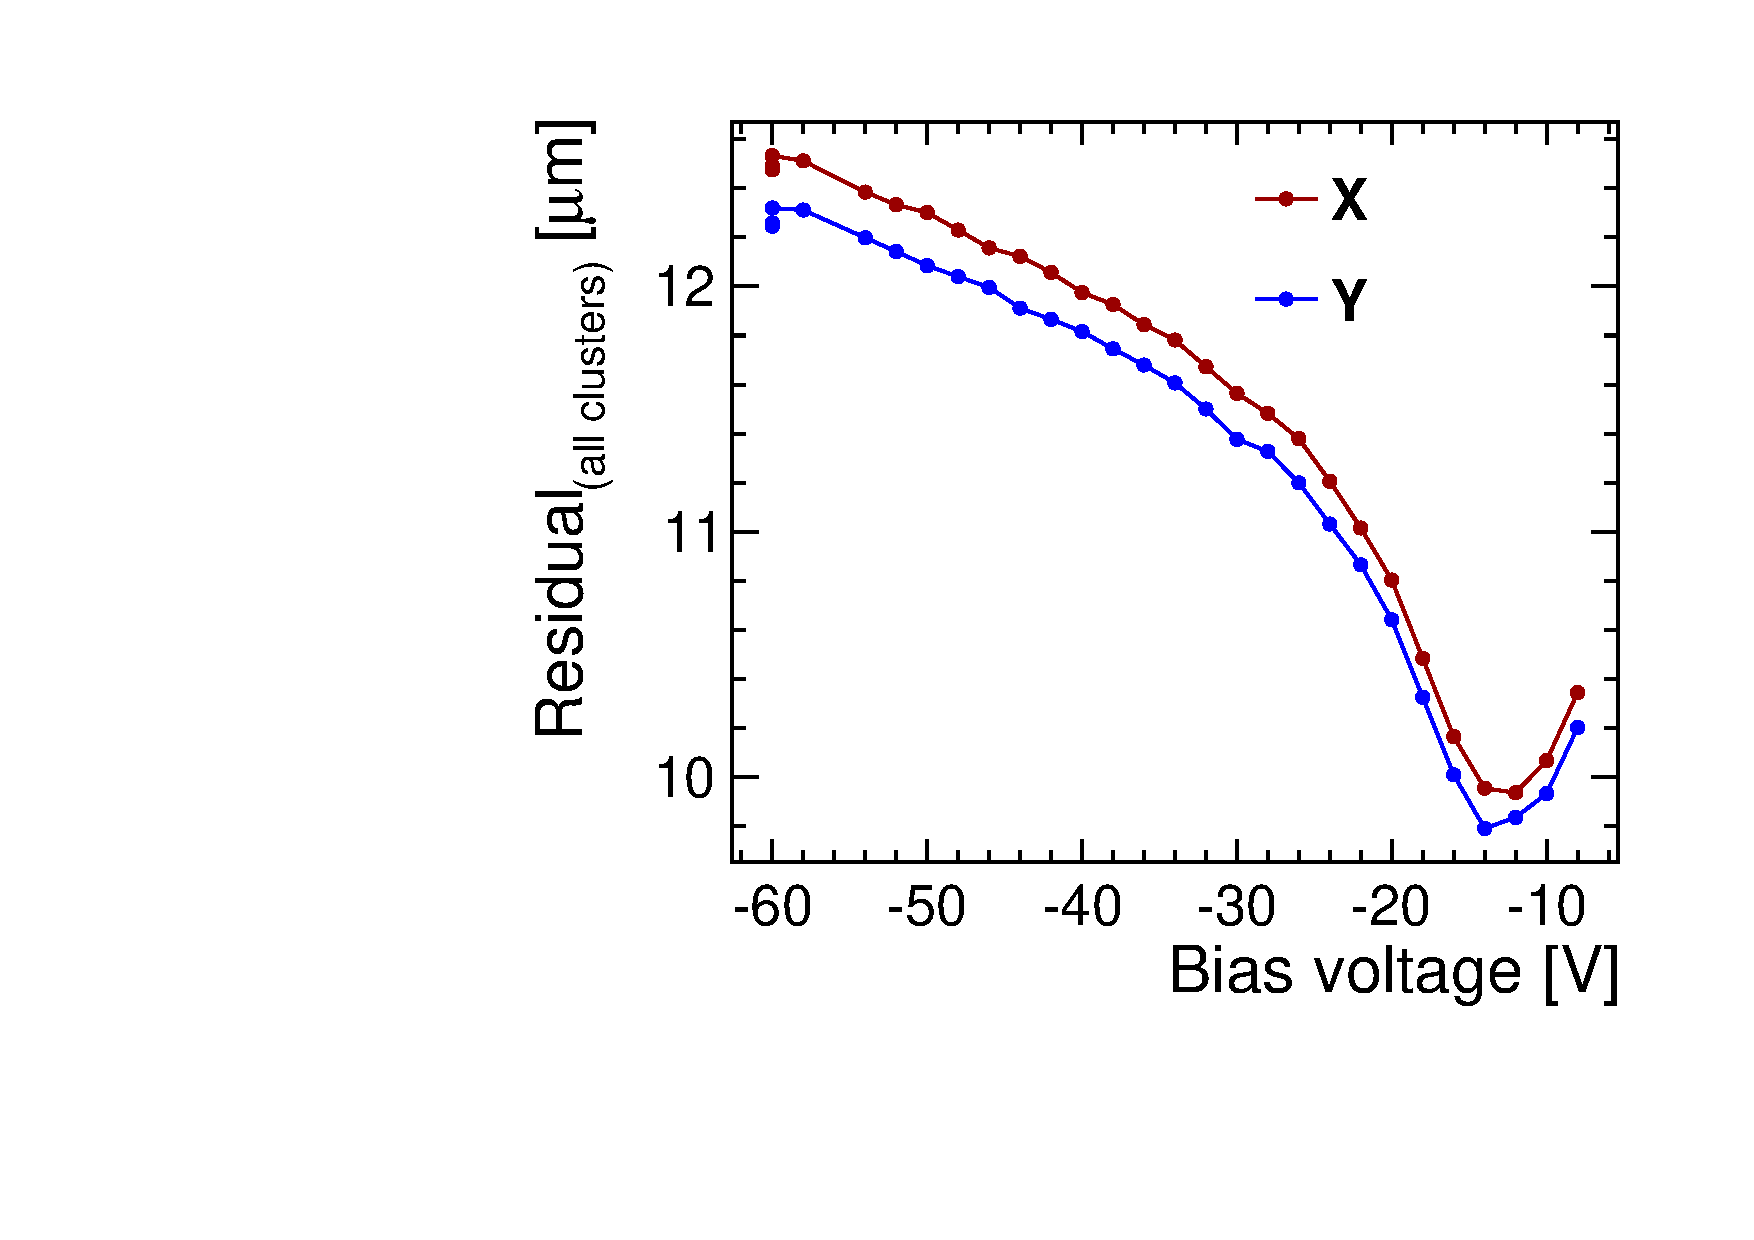
\includegraphics[width=\textwidth]{./figures/TestBeam/W5_F1_Residual_vs_bias.pdf}
    \caption{55-GND-GR-150}
  \end{subfigure}\\
  \begin{subfigure}[b]{0.33\textwidth}
    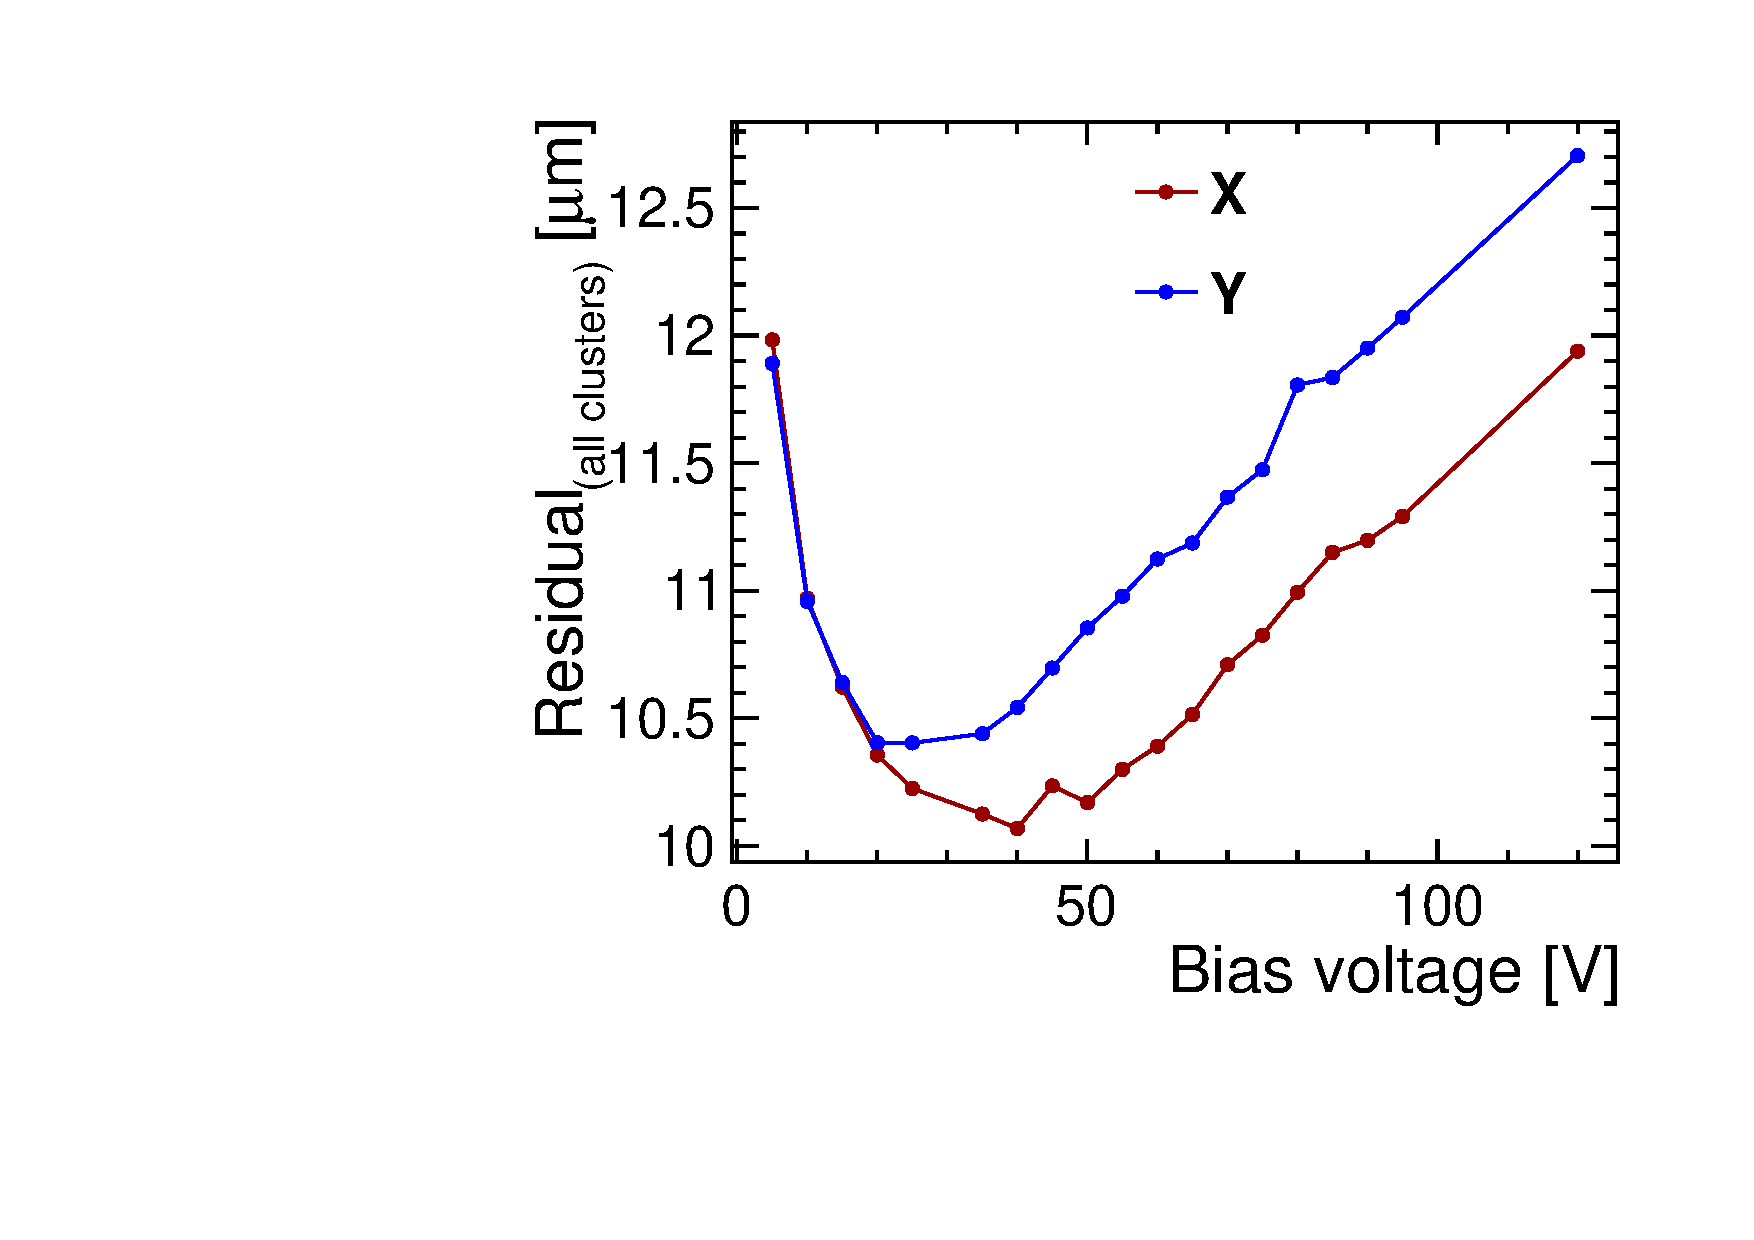
\includegraphics[width=\textwidth]{./figures/TestBeam/W2_J5_Residual_vs_bias.pdf}
    \caption{W2\_J5}
  \end{subfigure}
  \caption{Residuals vs. bias voltage.}
  \label{fig:Residuals_vs_biasVoltage}
\end{figure}

\newpage



%% \begin{figure}[htbp] \centering
%%   \begin{subfigure}[b]{0.45\textwidth}

%%     \caption{}
%%   \end{subfigure} \hfill
%%   \begin{subfigure}[b]{0.45\textwidth}
%%     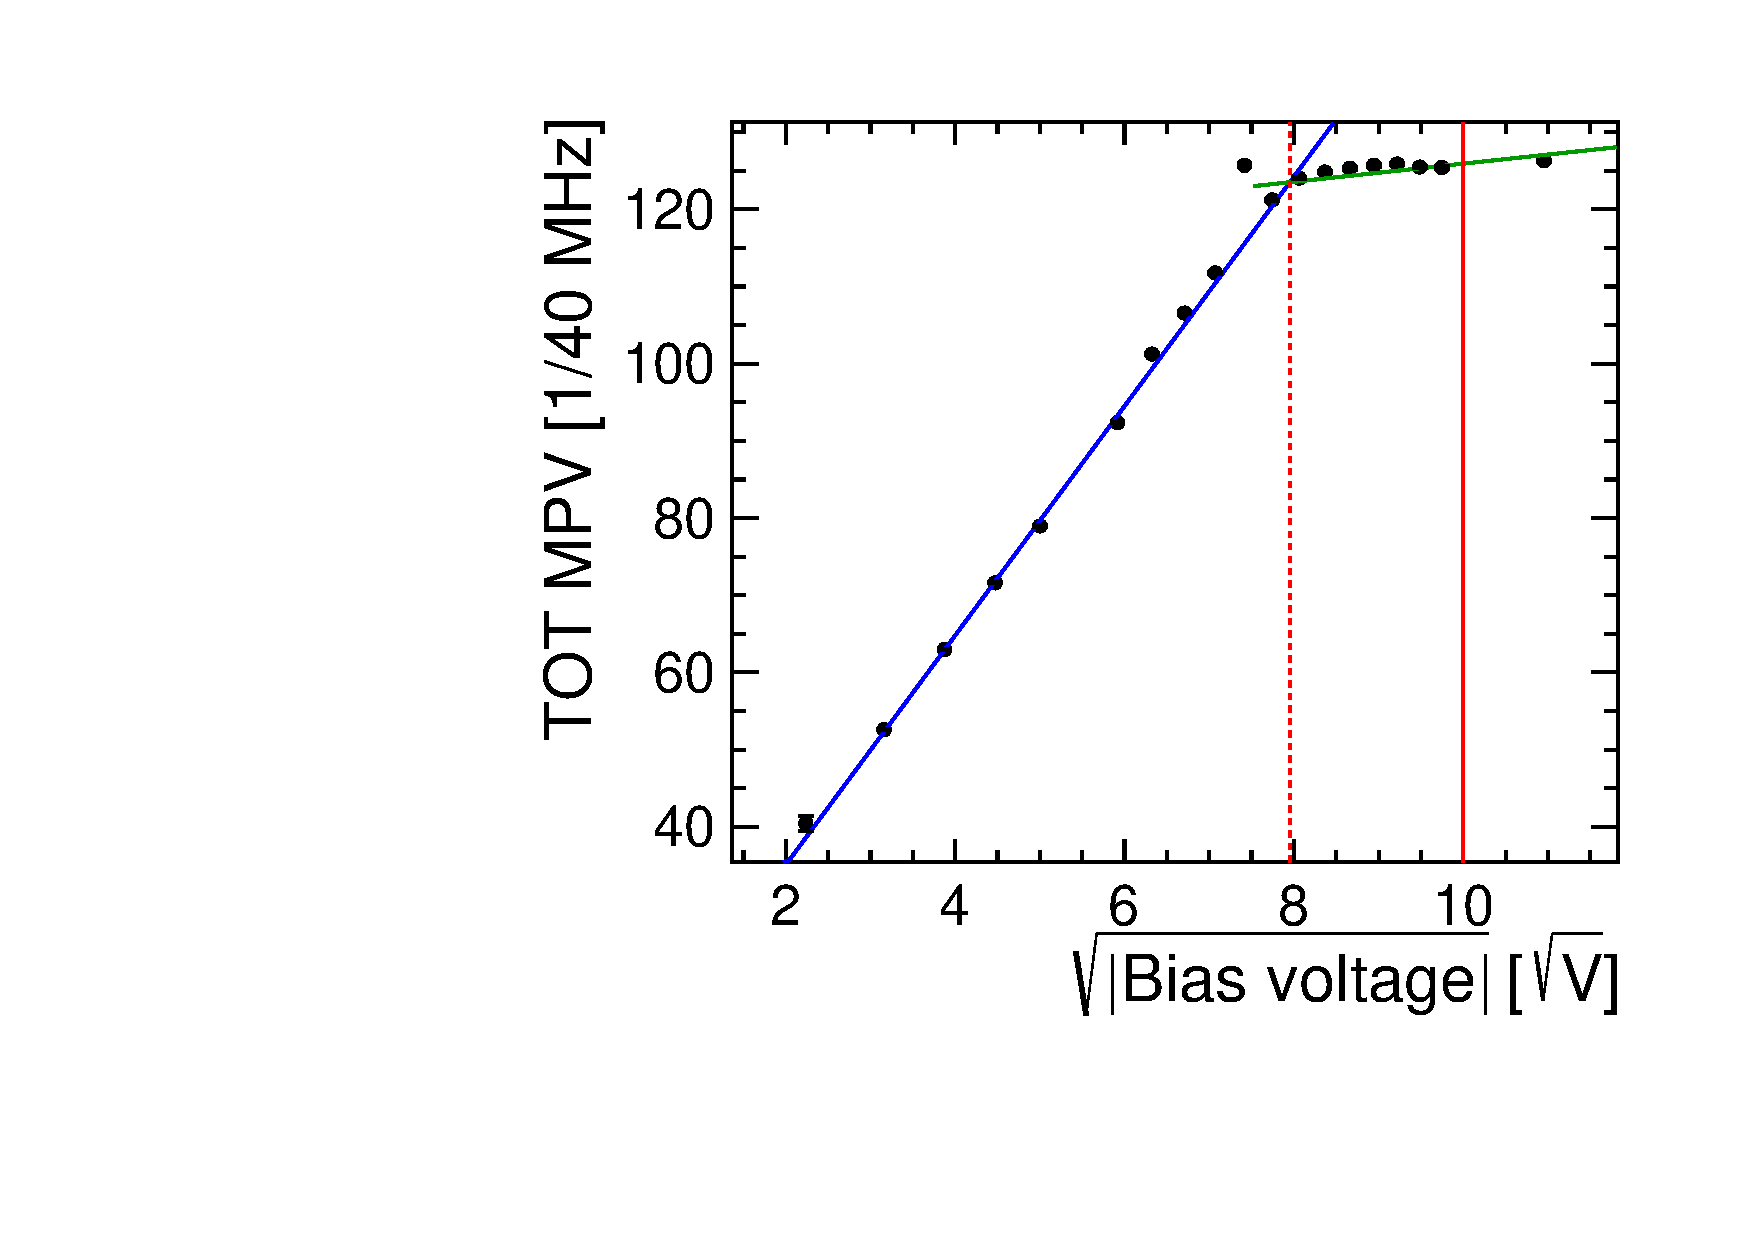
\includegraphics[width=\textwidth]{./figures/TestBeam/depletionVoltage_W0002_J05.pdf}
%%     \caption{}
%%   \end{subfigure}
%%   \caption{W2\_J5}
%%   \label{fig:W2_J5_depletion}
%% \end{figure}
